% --- ĐẦU FILE (Preamble) ---
\documentclass[a4paper,12pt]{report}
\usepackage[utf8]{inputenc}
\usepackage[T5]{fontenc}
\usepackage[vietnamese]{babel}
\usepackage{lmodern}
\usepackage{graphicx}
\usepackage{float}
\usepackage{geometry}
\usepackage{booktabs}
\usepackage{tabularx}
\usepackage{longtable}
\usepackage{caption}
\usepackage{subcaption}
\usepackage{hyperref}
\usepackage{setspace}
\usepackage{array}
\usepackage{placeins}
\usepackage{titlesec}
\usepackage{enumitem}
\setlist{nosep}
\usepackage{listings}
\usepackage{xcolor}
\usepackage{amsmath}
\usepackage{amssymb}
\usepackage{tikz}
\usepackage{microtype}

\geometry{a4paper, left=18mm, right=18mm, top=15mm, bottom=15mm}
\graphicspath{{./images/}}
\setstretch{1.10}
\raggedbottom
\titlespacing*{\chapter}{0pt}{-2cm}{0.5cm}

% Định nghĩa màu thương hiệu Viettel
\definecolor{ViettelRed}{HTML}{EE0033}

% Cấu hình code listing
\lstset{
    basicstyle=\ttfamily\small,
    breaklines=true,
    frame=single,
    backgroundcolor=\color{gray!8},
    numbers=left,
    numberstyle=\tiny\color{gray},
    numbersep=6pt,
    tabsize=4,
    showstringspaces=false,
    xleftmargin=1.5em,
    framexleftmargin=1.5em,
    literate=
      {á}{{\'a}}1 {à}{{\`a}}1 {ả}{{\d{a}}}1 {ã}{{\~a}}1 {ạ}{{\d{a}}}1
      {Á}{{\'A}}1 {À}{{\`A}}1 {Ả}{{\d{A}}}1 {Ã}{{\~A}}1 {Ạ}{{\d{A}}}1
      {đ}{{\dj{}}}1 {Đ}{{\DJ{}}}1
      {é}{{\'e}}1 {è}{{\`e}}1 {ẻ}{{\d{e}}}1 {ẽ}{{\~e}}1 {ẹ}{{\d{e}}}1
      {í}{{\'i}}1 {ì}{{\`i}}1 {ỉ}{{\d{i}}}1 {ĩ}{{\~i}}1 {ị}{{\d{i}}}1
      {ó}{{\'o}}1 {ò}{{\`o}}1 {ỏ}{{\d{o}}}1 {õ}{{\~o}}1 {ọ}{{\d{o}}}1
      {ú}{{\'u}}1 {ù}{{\`u}}1 {ủ}{{\d{u}}}1 {ũ}{{\~u}}1 {ụ}{{\d{u}}}1
      {ý}{{\'y}}1 {ỳ}{{\`y}}1 {ỷ}{{\d{y}}}1 {ỹ}{{\~y}}1 {ỵ}{{\d{y}}}1,
}

% Cấu hình hyperlink
\hypersetup{
    colorlinks=true,
    linkcolor=blue,
    urlcolor=blue,
    citecolor=blue
}
\usepackage{bookmark}

\begin{document}

% ==================== TRANG BÌA ====================
\begin{titlepage}
    \begin{tikzpicture}[remember picture, overlay]
        % Khung viền đôi màu đỏ thương hiệu Viettel
        \draw[line width=3pt, color=ViettelRed] 
            ([xshift=15mm, yshift=-13mm]current page.north west) 
            rectangle 
            ([xshift=-15mm, yshift=13mm]current page.south east);
        \draw[line width=1pt, color=ViettelRed] 
            ([xshift=15mm, yshift=-13mm]current page.north west) 
            rectangle 
            ([xshift=-15mm, yshift=13mm]current page.south east);
    \end{tikzpicture}

    \centering
    \vspace*{0.5cm}
    
    % Logo Viettel màu đỏ
    
\includegraphics[width=0.35\textwidth]{images/viettel_logo.png}\\[0.2cm]

    {\fontsize{14}{16}\selectfont \textbf{\color{ViettelRed}TẬP ĐOÀN CÔNG NGHIỆP -- VIỄN THÔNG QUÂN ĐỘI}}\\[0.15cm]
    {\fontsize{12}{14}\selectfont \textbf{VIETTEL HIGH TECH}}\\[1.2cm]
    
    \rule{0.7\textwidth}{1.5pt}\\[1.2cm]
    
    {\fontsize{26}{30}\selectfont \textbf{\color{ViettelRed}BÁO CÁO TỔNG KẾT DỰ ÁN}}\\[0.6cm]
    {\fontsize{22}{26}\selectfont \textbf{3DGS AR PIPELINE}}\\[0.5cm]
    {\fontsize{13}{16}\selectfont \textbf{Nghiên cứu và phát triển công cụ xử lý dữ liệu\\ 3D Gaussian Splatting phục vụ hệ thống Thực tế tăng cường (AR)}}\\[0.5cm]
    
    \rule{0.7\textwidth}{1.5pt}
    
    \vfill
    
    \begin{minipage}{0.85\textwidth}
        \large
        \renewcommand{\arraystretch}{1.3}
        \begin{tabular}{ll}
            \textbf{Hội đồng đánh giá:} & Hội đồng VDT 2026 / Toàn bộ hội đồng \\
            \textbf{Mentor hướng dẫn:}   & Hoàng Kim Đức \\
            \textbf{Cá nhân thực hiện:}   & Lê Việt Thành \\
            \textbf{Đơn vị:}             & Chương trình Viettel Digital Talent 2026 \\
        \end{tabular}
        \begin{tabular}{ll}
            \textbf{GitHub:}& \href{https://github.com/LeVietThanh1412/vdt-2026-3d-gaussian-splatting}{\texttt{LeVietThanh1412/vdt-2026-3d-gaussian-splatting}} \\
        \end{tabular}
    \end{minipage}\\[2.5cm]
    
    \large Hà Nội, tháng 07 năm 2026
\end{titlepage}

% ==================== LỜI MỞ ĐẦU ====================
\chapter*{Lời mở đầu}
\addcontentsline{toc}{chapter}{Lời mở đầu}
\markboth{Lời mở đầu}{Lời mở đầu}

Trong kỷ nguyên số hóa mạnh mẽ và sự phát triển vượt bậc của công nghệ máy tính, việc tái cấu trúc và số hóa không gian ba chiều (3D) đang trở thành một trong những lĩnh vực nghiên cứu sôi nổi nhất của thị giác máy tính (Computer Vision) và đồ họa máy tính (Computer Graphics). Các công nghệ như Thực tế tăng cường (AR - Augmented Reality) và Thực tế ảo (VR - Virtual Reality) đang chuyển mình từ những ứng dụng giải trí đơn thuần sang các công cụ cốt lõi trong nhiều ngành công nghiệp như thương mại điện tử, y tế, giáo dục, quốc phòng và xây dựng đô thị thông minh.

Một trong những thách thức lớn nhất của việc đưa thế giới thực vào không gian số là làm thế nào để tái tạo lại các cảnh quan thực tế một cách nhanh chóng, chân thực mà vẫn đảm bảo hiệu suất hiển thị thời gian thực (real-time rendering). Trước đây, Neural Radiance Fields (NeRF) đã mở ra một hướng đi đầy hứa hẹn nhờ khả năng mô hình hóa trường ánh sáng phức tạp thông qua các mạng thần kinh nhân tạo. Tuy nhiên, điểm yếu cố hữu của NeRF là tốc độ dựng hình (rendering speed) cực kỳ chậm do phải thực hiện truy vấn mạng thần kinh liên tục cho từng tia sáng đi qua không gian.

Sự xuất hiện của kỹ thuật 3D Gaussian Splatting (3DGS) vào cuối năm 2023 đã tạo nên một bước ngoặt lịch sử. Bằng cách sử dụng hàng triệu hạt Gaussian ba chiều để biểu diễn cảnh vật và áp dụng giải thuật rasterization phân mảnh nhanh (fast tile-based rasterizer), 3DGS cho phép dựng hình với tốc độ hàng trăm khung hình trên giây (FPS) ở độ phân giải cực cao mà vẫn giữ được độ chân thực vượt trội.

Tuy nhiên, dữ liệu đầu ra của 3DGS thường là một tập hợp khổng lồ các hạt Gaussian rời rạc, có dung lượng cực lớn (từ vài trăm Megabytes đến hàng Gigabytes) và không có cấu trúc bề mặt dạng lưới tam giác truyền thống (polygonal mesh). Điều này khiến việc hiển thị trực tiếp dữ liệu 3DGS trên các thiết bị di động cấu hình yếu hoặc tích hợp vào các engine AR phổ biến (như Unity, Unreal Engine, WebXR) gặp vô vàn khó khăn về băng thông mạng, bộ nhớ RAM và hiệu suất xử lý của GPU.

Nhận thức được bài toán thực tiễn này, dự án "3DGS AR Pipeline" được ra đời nhằm nghiên cứu và phát triển một hệ thống tự động hóa hoàn chỉnh để chuyển đổi, lọc nhiễu, tối ưu hóa và trích xuất dữ liệu 3DGS thành các mô hình lưới 3D có cấu trúc, dung lượng nhẹ, hỗ trợ che khuất (Occlusion) và điều hướng (Navigation) tương thích tốt với các tiêu chuẩn đồ họa AR hiện nay. Báo cáo này trình bày chi tiết từ cơ sở lý thuyết, kiến trúc hệ thống, chi tiết triển khai phần mềm cho đến kết quả thực nghiệm và những đánh giá định lượng về hiệu năng của pipeline.

Tác giả xin gửi lời cảm ơn chân thành đến Tập đoàn Công nghiệp - Viễn thông Quân đội (Viettel) đã tạo điều kiện và môi trường học tập, nghiên cứu tuyệt vời trong chương trình Viettel Digital Talent 2026. Xin chân thành cảm ơn Ban tổ chức chương trình VDT 2026, toàn thể quý anh/chị mentor trong Hội đồng đánh giá đã dành thời gian quý báu để phản biện và đóng góp ý kiến cho dự án.

% ==================== Nội dung thực hiện ====================mentor
\chapter*{Nội dung thực hiện}
\addcontentsline{toc}{chapter}{Nội dung thực hiện}
\markboth{Nội dung thực hiện}{Nội dung thực hiện}

\begin{enumerate}[label=\arabic*.]
    \item \textbf{Nghiên cứu lý thuyết và lựa chọn giải thuật:} Khảo sát và đánh giá toàn diện các kỹ thuật xử lý hình học 3D, từ các giải thuật lọc nhiễu thống kê đám mây điểm (SOR), tái tạo bề mặt ngầm (Poisson Surface Reconstruction) cho đến các phương pháp thu gọn lưới bảo toàn đặc tính hình học (QEM).
    \item \textbf{Thiết kế kiến trúc hệ thống:} Xây dựng kiến trúc đường ống xử lý (pipeline) gồm 6 giai đoạn độc lập, có tính module hóa cao, dễ dàng mở rộng và tối ưu hóa độc lập. Thiết kế các kiểu dữ liệu cốt lõi giúp tối ưu hóa việc truyền và lưu trữ thông tin giữa các giai đoạn.
    \item \textbf{Lập trình hệ thống hiệu năng cao bằng C++17:} Hiện thực hóa pipeline dưới dạng một công cụ dòng lệnh (CLI) bằng ngôn ngữ C++17. Tận dụng tối đa sức mạnh tính toán của các thư viện mã nguồn mở hàng đầu như Open3D, tinygltf, happly và CLI11 để đảm bảo tốc độ xử lý nhanh nhất và quản lý bộ nhớ an toàn.
    \item \textbf{Phát triển giải thuật phân loại AR:} Đề xuất và triển khai thuật toán phân tách lưới tam giác tự động dựa trên hướng của vector pháp tuyến so với trục trọng lực, giúp tách biệt chính xác lưới che khuất vật thể ảo (Occlusion Mesh) và lưới điều hướng di chuyển (Navigation Mesh).
    \item \textbf{Đóng gói và triển khai container hóa:} Thiết lập hệ thống biên dịch tự động bằng CMake và đóng gói toàn bộ ứng dụng bằng Docker và Docker Compose, giúp chạy thử nghiệm pipeline dễ dàng trên mọi môi trường mà không lo ngại về xung đột thư viện phụ thuộc.
    \item \textbf{Xây dựng Web Demo tương tác:} Thiết kế giao diện web tương tác sử dụng component \texttt{<model-viewer>} của Google, hỗ trợ trực quan hóa mô hình 3D và thử nghiệm tính năng thực tế tăng cường (AR) thông qua WebXR và AR Quick Look trên các thiết bị di động thực tế.
    \item \textbf{Đánh giá thực nghiệm:} Thực hiện các thực nghiệm định lượng trên các bộ dữ liệu 3DGS công khai có kích thước khác nhau (như ChristmasTree và Flowers), đo lường chi tiết hiệu suất nén, thời gian chạy của từng module và chất lượng lưới đầu ra để chứng minh tính thực tiễn của giải pháp.
\end{enumerate}

\newpage

% ==================== MỤC LỤC & DANH MỤC ====================
\tableofcontents
\newpage
\listoffigures
\listoftables
\newpage

% ==================== CHƯƠNG 1 ====================
\chapter{Tổng quan dự án}

\section{Bối cảnh và động lực}
Trong bối cảnh công nghệ Thực tế tăng cường (AR) phát triển nhanh, nhu cầu đưa mô hình 3D chân thực vào không gian số ngày càng rõ rệt trong thương mại điện tử, giáo dục và công nghiệp. Việc chụp quét và tái tạo lại các đối tượng, cảnh quan từ thế giới thực (Real-world 3D Reconstruction) đóng vai trò then chốt trong việc tạo ra nội dung số chất lượng cao. Kỹ thuật \textbf{3D Gaussian Splatting (3DGS)} nổi lên như một hướng tiếp cận mới đầy hứa hẹn cho tái tạo cảnh 3D chất lượng cao từ ảnh 2D, với tốc độ dựng hình tốt hơn nhiều so với Neural Radiance Fields (NeRF).

Tuy nhiên, dữ liệu đầu ra của 3DGS thường là một tập hợp khổng lồ các hạt Gaussian rời rạc, có kích thước lớn, không có cấu trúc mặt và chưa thể sử dụng trực tiếp trong các nền tảng AR truyền thống. Các framework AR trên thiết bị di động thường yêu cầu định dạng hình học dạng lưới tam giác chuẩn (Polygonal Mesh) cùng với chất liệu (Material) hoặc màu sắc đỉnh (Vertex Colors). Vì vậy, cần một pipeline tự động để lọc, tái tạo, tối ưu và xuất dữ liệu sang định dạng phù hợp cho AR.

\section{Bài toán đặt ra}
Dự án hướng tới việc nghiên cứu và phát triển một công cụ phần mềm tự động có khả năng chuyển đổi dữ liệu 3DGS dạng \texttt{.ply} thành lưới 3D có cấu trúc, nhẹ và phù hợp cho hiển thị AR trên các thiết bị di động thông thường. Hệ thống cần tự động nhận diện hướng không gian, tách riêng các vùng phục vụ che khuất (Occlusion Mesh) và điều hướng (Navigation Mesh).

Việc chuyển đổi từ tập hợp hạt Gaussian (với các thông tin bất đối xứng về tỷ lệ, hướng xoay và độ đục) sang một lưới tam giác liên tục đòi hỏi các giải thuật hình học phức tạp. Hệ thống phải giải quyết đồng thời việc loại bỏ nhiễu, ước lượng trường pháp tuyến, giải phương trình Poisson để dựng mặt, rút gọn số lượng tam giác mà vẫn giữ vững hình dáng cốt lõi, và cuối cùng là phân chia bề mặt vật lý dựa trên phân tích vector pháp tuyến.
page
\clearpage
\section{Yêu cầu chức năng}
Hệ thống cần đáp ứng đầy đủ các chức năng cốt lõi sau:
\begin{enumerate}
    \item \textbf{Đọc dữ liệu PLY:} Hỗ trợ tải các tệp tin \texttt{.ply} chứa dữ liệu đám mây điểm Gaussian từ các công cụ huấn luyện 3DGS chuẩn.
    \item \textbf{Tiền xử lý và lọc dữ liệu:} Lọc bỏ các hạt Gaussian không hợp lệ (NaN), các hạt có độ đục quá thấp, kích thước quá lớn, và các điểm cô lập ngoài biên (Outliers).
    \item \textbf{Ước lượng pháp tuyến:} Tính toán vector pháp tuyến cho tập hợp điểm đã lọc dựa trên cấu trúc láng giềng.
    \item \textbf{Tái tạo bề mặt (Surface Reconstruction):} Sử dụng thuật toán tái tạo bề mặt Poisson để tạo ra lưới tam giác kín từ đám mây điểm có hướng.
    \item \textbf{Tối ưu hóa lưới (Mesh Optimization):} Thực hiện rút gọn lưới tam giác bằng phương pháp sai số bậc hai (QEM) để giảm dung lượng file và số đa giác phù hợp với phần cứng di động.
    \item \textbf{Trích xuất và phân loại AR:} Tự động phân tích góc dốc của từng tam giác để gắn nhãn và phân chia thành Lưới điều hướng (Navigation Mesh) và Lưới che khuất (Occlusion Mesh).
    \item \textbf{Xuất tệp tin GLB:} Đóng gói mô hình dưới dạng tệp nhị phân \texttt{.glb} duy nhất chứa đầy đủ cấu trúc phân cấp đồ họa đồ thị (Scene Graph).
\end{enumerate}

\section{Yêu cầu phi chức năng}
\begin{enumerate}
    \item \textbf{Hiệu năng xử lý:} Pipeline phải xử lý các tệp tin đầu vào lớn (trên 500 MB) trong thời gian hợp lý (dưới 5 phút đối với cấu hình CPU tiêu chuẩn).
    \item \textbf{Khả năng nén dữ liệu:} Dung lượng tệp tin GLB đầu ra phải đạt mức tối ưu cao (giảm trên 90\% so với tệp PLY gốc), lý tưởng nhất là dưới 5 MB để truyền tải mượt mà qua Internet.
    \item \textbf{Độ trung thực hình học (Fidelity):} Giữ đúng tỷ lệ kích thước thật và hệ tọa độ của không gian quét ban đầu, không làm biến dạng cấu trúc hình học chính.
    \item \textbf{Tính di động và độc lập:} Phần mềm được đóng gói dưới dạng công cụ dòng lệnh (CLI) chạy trong môi trường Docker, không yêu cầu cài đặt thủ công các phụ thuộc phức tạp.
\end{enumerate}

% ==================== CHƯƠNG 2 ====================
\chapter{Phân công nhiệm vụ}

\section{Thành viên và vai trò}
Dự án được thực hiện độc lập bởi một cá nhân. Phạm vi công việc bao gồm toàn bộ các khâu từ nghiên cứu thuật toán lý thuyết, thiết kế kiến trúc hệ thống, phát triển mã nguồn C++, biên dịch, đóng gói container cho đến xây dựng ứng dụng web demo.

\begin{table}[H]
\centering
\small
\setlength{\tabcolsep}{6pt}
\renewcommand{\arraystretch}{1.3}
\begin{tabularx}{\textwidth}{|>{\centering\arraybackslash}p{0.08\textwidth}|>{\centering\arraybackslash}p{0.25\textwidth}|>{\raggedright\arraybackslash}X|}
\hline
\textbf{STT} & \textbf{Vai trò} & \textbf{Chi tiết công việc} \\ \hline
1 & \parbox[t]{0.25\textwidth}{\centering Lê Việt Thành\\--\\Tác giả dự án} &
\parbox[t]{\linewidth}{
- Nghiên cứu sâu lý thuyết 3D Gaussian Splatting và các thuật toán hình học 3D.\\
- Thiết kế kiến trúc tổng thể của pipeline 6 giai đoạn và định nghĩa các kiểu dữ liệu.\\
- Lập trình toàn bộ mã nguồn C++ của công cụ \texttt{gsplat\_ar}.\\
- Xây dựng tệp tin cấu hình CMake, thiết lập môi trường build tự động qua vcpkg.\\
- Thiết lập Dockerfile và Docker Compose cho quá trình chạy và thử nghiệm.\\
- Xây dựng trang Web Demo hỗ trợ hiển thị 3D và tương tác AR bằng WebXR.\\
- Thực hiện kiểm thử đơn vị, đo lường hiệu năng và viết báo cáo tổng kết.
} \\ \hline
\end{tabularx}
\normalsize
\caption{Bảng phân công nhiệm vụ chi tiết}
\label{tab:bang_phan_cong}
\end{table}

\clearpage
\section{Kế hoạch triển khai dự án}
Dự án được chia thành các mốc thời gian (Milestones) cụ thể để đảm bảo tiến độ:
\begin{itemize}
    \item \textbf{Step 1 - Nghiên cứu lý thuyết:} Đọc và hiểu cơ chế biểu diễn hạt của 3DGS, cách trích xuất tham số toán học từ file PLY. Lựa chọn các thuật toán phù hợp cho từng giai đoạn xử lý.
    \item \textbf{Step 2 - Thiết kế kiến trúc:} Định nghĩa các kiểu dữ liệu cốt lõi trong \texttt{types.hpp}. Thiết kế giao diện lập trình ứng dụng (API) cho từng module từ Stage 1 đến Stage 6.
    \item \textbf{Step 3 - Hiện thực hóa Core Pipeline:} Viết mã nguồn C++ cho việc đọc file PLY bằng \texttt{happly}, lọc điểm bằng giải thuật SOR của Open3D, dựng mặt bằng Poisson và tối ưu hóa lưới bằng QEM.
    \item \textbf{Step 4 - AR Extraction và Exporter:} Phát triển thuật toán phân loại tam giác dựa trên pháp tuyến và xuất mô hình nhị phân GLB bằng thư viện \texttt{tinygltf}.
    \item \textbf{Step 5 - Web Demo và Đóng gói:} Thiết kế trang web demo, cấu hình Docker cho toàn bộ dự án. Viết các kịch bản unit test.
    \item \textbf{Step 6 - Thực nghiệm và Tối ưu:} Chạy thử nghiệm trên các bộ dữ liệu thực tế, đo đạc thời gian xử lý, tối ưu hóa các tham số mặc định và hoàn thiện báo cáo.
\end{itemize}

% ==================== CHƯƠNG 3 ====================
\chapter{Cơ sở lý thuyết}

\section{3D Gaussian Splatting (3DGS)}
3D Gaussian Splatting biểu diễn không gian 3D bằng một tập hợp các hàm mật độ xác suất Gaussian 3D. Mỗi hạt Gaussian được đặc trưng bởi các thuộc tính hình học và quang học. Công thức toán học biểu diễn một hạt Gaussian 3D tại vị trí $x \in \mathbb{R}^3$ là:
\begin{equation}
    G(x) = \exp\left(-\frac{1}{2} (x-\mu)^T \Sigma^{-1} (x-\mu)\right)
\end{equation}
Trong đó:
\begin{itemize}
    \item $\mu = (x, y, z)$ là vector kỳ vọng, đại diện cho tọa độ tâm của hạt Gaussian trong không gian 3D.
    \item $\Sigma$ là ma trận hiệp phương sai 3D, quyết định hình dạng và hướng của hạt Gaussian.
\end{itemize}

Để đảm bảo ma trận hiệp phương sai $\Sigma$ luôn là ma trận xác định dương (positive definite) trong quá trình tối ưu hóa gradient descent, người ta phân tích $\Sigma$ thành tích của ma trận xoay $R$ và ma trận tỷ lệ $S$:
\begin{equation}
    \Sigma = R S S^T R^T
\end{equation}
Trong đó:
\begin{itemize}
    \item $S = \text{diag}(s_x, s_y, s_z)$ là ma trận đường chéo chứa các hệ số tỷ lệ dọc theo ba trục chính. Trong file PLY gốc, các giá trị này được lưu dưới dạng logarit cơ số tự nhiên nhằm tránh giá trị âm. Do đó, khi đọc dữ liệu ta cần giải nén bằng hàm mũ:
    \begin{equation}
        s_{\text{actual}} = e^{s_{\text{raw}}}
    \end{equation}
    \item $R$ là ma trận xoay thu được từ một quaternion đơn vị $q = (w, x, y, z)$. Công thức chuyển đổi từ quaternion sang ma trận xoay $R(q)$ là:
    \begin{equation}
        R(q) = \begin{bmatrix} 
        1 - 2(y^2+z^2) & 2(xy-wz) & 2(xz+wy) \\ 
        2(xy+wz) & 1 - 2(x^2+z^2) & 2(yz-wx) \\ 
        2(xz-wy) & 2(yz+wx) & 1 - 2(x^2+y^2) 
        \end{bmatrix}
    \end{equation}
\end{itemize}

Ngoài ra, mỗi hạt Gaussian còn chứa thông tin về độ đục $\alpha$, được lưu dưới dạng giá trị logit thô $\alpha_{\text{raw}}$ và được chuyển đổi sang miền $[0,1]$ bằng hàm sigmoid:
\begin{equation}
    \alpha_{\text{actual}} = \sigma(\alpha_{\text{raw}}) = \frac{1}{1 + e^{-\alpha_{\text{raw}}}}
\end{equation}

Thông tin màu sắc phụ thuộc vào hướng nhìn được biểu diễn thông qua các hệ số hài cầu (Spherical Harmonics - SH). Hệ số hài cầu bậc 0 đại diện cho màu sắc cơ bản (màu khuếch tán - diffuse color). Chuyển đổi từ hệ số SH bậc 0 ($f_{\text{dc\_0}}, f_{\text{dc\_1}}, f_{\text{dc\_2}}$) sang giá trị màu RGB thô trong đoạn $[0, 1]$ được thực hiện qua công thức tuyến tính hóa:
\begin{equation}
    C_{\text{RGB}} = 0.5 + 0.28209 \times f_{\text{dc}}
\end{equation}

\section{Statistical Outlier Removal (SOR)}
Thuật toán SOR được áp dụng để loại bỏ các hạt Gaussian cô lập, thường là kết quả của nhiễu trong quá trình huấn luyện hoặc các hạt trôi nổi tự do trong không gian không thuộc về bề mặt thực tế của vật thể.
\begin{enumerate}
    \item Với mỗi điểm $p_i$ trong đám mây điểm, thuật toán sử dụng cấu trúc KD-Tree để tìm kiếm nhanh $k$ điểm láng giềng gần nhất.
    \item Tính toán khoảng cách trung bình $d_i$ từ điểm $p_i$ tới toàn bộ $k$ láng giềng đó:
    \begin{equation}
        d_i = \frac{1}{k} \sum_{p_j \in N(p_i)} \|p_i - p_j\|
    \end{equation}
    \item Tính toán giá trị trung bình $\mu_d$ và độ lệch chuẩn $\sigma_d$ của tập hợp khoảng cách trung bình của toàn bộ đám mây điểm chứa $N$ điểm:
    \begin{equation}
        \mu_d = \frac{1}{N} \sum_{i=1}^N d_i, \quad \sigma_d = \sqrt{\frac{1}{N} \sum_{i=1}^N (d_i - \mu_d)^2}
    \end{equation}
    \item Một điểm $p_i$ bị coi là điểm ngoại lai (outlier) và bị loại bỏ nếu khoảng cách trung bình của nó vượt quá ngưỡng cắt lọc thống kê:
    \begin{equation}
        d_i > \mu_d + \beta \cdot \sigma_d
    \end{equation}
    Trong đó $\beta$ là hệ số nhân độ lệch chuẩn (thường chọn từ 1.0 đến 3.0).
\end{enumerate}

\section{Poisson Surface Reconstruction}
Tái tạo bề mặt Poisson là phương pháp dựng lưới tam giác ngầm từ đám mây điểm có hướng (Point Cloud với các vector pháp tuyến). Thuật toán coi bài toán dựng mặt là một bài toán biên giải phương trình Poisson.

Giả sử có mô hình 3D kín $M$ với bề mặt biên $\partial M$. Hàm chỉ thị $\chi_M$ được định nghĩa bằng 1 cho các điểm nằm trong $M$ và bằng 0 cho các điểm nằm ngoài $M$. Gradient của hàm chỉ thị $\nabla \dots$ bằng không ở hầu hết mọi nơi, ngoại trừ ở khu vực gần bề mặt biên $\partial M$, nơi nó hướng vào phía trong và có độ lớn tương đương vector pháp tuyến bề mặt.

Do đó, trường vector pháp tuyến định hướng $V$ thu được từ đám mây điểm có thể coi là xấp xỉ của gradient của hàm chỉ thị:
\begin{equation}
    \nabla \chi \approx V
\end{equation}
Để tìm hàm chỉ thị $\chi$ tốt nhất từ mối quan hệ này, ta áp dụng toán tử divergence $\nabla \cdot$ lên cả hai vế, chuyển nó thành phương trình Poisson:
\begin{equation}
    \nabla^2 \chi = \nabla \cdot V
\end{equation}
Thuật toán giải phương trình này bằng phương pháp số trên cấu trúc phân cấp Octree với độ sâu $d$. Độ sâu octree quyết định độ phân giải chi tiết của lưới tam giác đầu ra. Sau khi giải được hàm $\chi$, bề mặt lưới $\partial M$ được trích xuất bằng giải thuật Marching Cubes tại mức giá trị đẳng trị (iso-value).

\section{Quadric Error Metrics (QEM)}
Sau khi dựng mặt, số lượng tam giác thường rất lớn. Thuật toán QEM rút gọn lưới dựa trên việc thực hiện liên tiếp phép co cạnh (edge collapse). Mỗi phép co cạnh $(v_1, v_2) \rightarrow \bar{v}$ sẽ gộp hai đỉnh thành một đỉnh mới.

Sai số hình học tại một đỉnh $v = [x, y, z, 1]^T$ được đo bằng tổng bình phương khoảng cách từ đỉnh đó tới tập hợp các mặt phẳng $P$ chứa các tam giác xung quanh đỉnh đó:
\begin{equation}
    \Delta(v) = \sum_{p \in P} (p^T v)^2 = v^T \left( \sum_{p \in P} p p^T \right) v = v^T Q v
\end{equation}
Trong đó $p = [a, b, c, d]^T$ đại diện cho phương trình mặt phẳng $ax + by + cz + d = 0$ với điều kiện chuẩn hóa $a^2 + b^2 + c^2 = 1$. Ma trận $Q$ là ma trận lỗi bậc hai kích thước $4 \times 4$ đối xứng:
\begin{equation}
    Q = \sum_{p \in P} \begin{bmatrix}
    a^2 & ab & ac & ad \\
    ab & b^2 & bc & bd \\
    ac & bc & c^2 & cd \\
    ad & bd & cd & d^2
    \end{bmatrix}
\end{equation}

Khi thực hiện co cạnh $(v_1, v_2)$ thành $\bar{v}$, ma trận lỗi bậc hai của đỉnh mới là:
\begin{equation}
    \bar{Q} = Q_1 + Q_2
\end{equation}
Vị trí tối ưu của $\bar{v}$ được lựa chọn bằng cách giải hệ phương trình đạo hàm riêng bằng không để cực tiểu hóa sai số $\bar{v}^T \bar{Q} \bar{v}$:
\begin{equation}
    \begin{bmatrix}
    q_{11} & q_{12} & q_{13} & q_{14} \\
    q_{12} & q_{22} & q_{23} & q_{24} \\
    q_{13} & q_{23} & q_{33} & q_{34} \\
    0 & 0 & 0 & 1
    \end{bmatrix} \bar{v} = \begin{bmatrix} 0 \\ 0 \\ 0 \\ 1 \end{bmatrix}
\end{equation}
Nếu ma trận không khả nghịch, ta chọn $\bar{v}$ là trung điểm hoặc một trong hai đầu mút $v_1, v_2$ dựa trên sai số nhỏ nhất.

\section{Phân loại mặt tam giác cho AR}
Để tích hợp mượt mà vào AR, ta cần phân tách lưới hình học thành hai thành phần vật lý riêng biệt dựa trên vector pháp tuyến mặt $\vec{n} = (n_x, n_y, n_z)$.
Giả sử vector trọng lực hướng thẳng đứng lên trên được định nghĩa là $\vec{u}_{\text{up}} = (0, 1, 0)$ (trong hệ tọa độ Right-handed chuẩn của OpenGL/glTF). Góc dốc $\theta$ của tam giác so với mặt nằm ngang được xác định qua tích vô hướng:
\begin{equation}
    \cos\theta = \frac{\vec{n} \cdot \vec{u}_{\text{up}}}{\|\vec{n}\| \|\vec{u}_{\text{up}}\|} = n_y
\end{equation}
\begin{equation}
    \theta = \arccos(|n_y|) \times \frac{180}{\pi}
\end{equation}
Nếu $\theta \le \theta_{\text{slope}}$ (ngưỡng góc dốc, mặc định là $45^\circ$), mặt tam giác được phân loại là mặt nằm ngang phẳng, thuộc về \textbf{Navigation Mesh}.
Ngược lại, nếu $\theta > \theta_{\text{slope}}$, mặt tam giác được đưa vào nhóm các mặt đứng, dốc đứng, đóng vai trò làm vật cản vật lý hoặc che chắn không gian ảo, thuộc về \textbf{Occlusion Mesh}.

% ==================== CHƯƠNG 4 ====================
\chapter{Kiến trúc và thiết kế hệ thống}

\section{Kiến trúc tổng thể pipeline}
Hệ thống được thiết kế theo kiến trúc đường ống xử lý tuần tự (Sequential Pipeline Architecture) gồm 6 giai đoạn rõ ràng. Mỗi giai đoạn đại diện cho một module xử lý chuyên biệt, nhận dữ liệu từ giai đoạn trước và cung cấp dữ liệu đầu ra cho giai đoạn tiếp theo.

\begin{figure}[H]
    \centering
    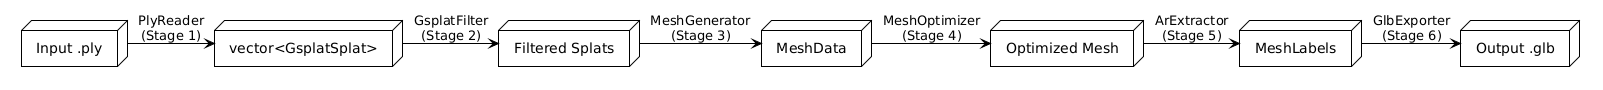
\includegraphics[width=0.95\textwidth]{pipeline.png}
    \caption{Sơ đồ luồng xử lý 6 giai đoạn của hệ thống 3DGS AR Pipeline}
    \label{fig:pipeline_architecture}
\end{figure}

Luồng hoạt động tuần tự như sau:
\begin{enumerate}
    \item \textbf{Stage 1 -- PlyReader:} Tải file dữ liệu PLY thô từ đĩa cứng. Tiến hành giải nén cấu trúc nhị phân và đọc các thuộc tính của hạt Gaussian, thực hiện ánh xạ sigmoid cho độ đục và chuyển đổi màu sắc từ hài cầu sang RGB cơ bản.
    \item \textbf{Stage 2 -- GsplatFilter:} Nhận danh sách hạt Gaussian từ PlyReader. Lọc bỏ các hạt chứa giá trị lỗi NaN, hạt quá mờ (độ đục nhỏ hơn ngưỡng $\alpha_{\text{min}}$), hạt có kích thước quá lớn (scale vượt ngưỡng $S_{\text{max}}$). Sau đó áp dụng thuật toán lọc SOR để loại bỏ nhiễu biên.
    \item \textbf{Stage 3 -- MeshGenerator:} Chuyển đổi đám mây điểm đã lọc sang lưới tam giác. Bước này bao gồm tính toán trường pháp tuyến cho các hạt, dựng mặt kín bằng Poisson Reconstruction, loại bỏ các đỉnh ở vùng có mật độ phân bố điểm cực thấp, và gán lại màu sắc đỉnh bằng phương pháp nội suy KNN từ đám mây điểm gốc.
    \item \textbf{Stage 4 -- MeshOptimizer:} Nhận lưới tam giác mật độ cao từ MeshGenerator. Thực hiện giải thuật rút gọn QEM để giảm số lượng đa giác về ngưỡng mục tiêu, dọn dẹp các tam giác suy biến và đỉnh cô lập, tính toán lại vector pháp tuyến đỉnh để chuẩn bị xuất file.
    \item \textbf{Stage 5 -- ArExtractor:} Phân tích cấu trúc lưới tam giác. Duyệt qua toàn bộ danh sách mặt tam giác, tính toán vector pháp tuyến mặt, thực hiện tích vô hướng với trục trọng lực và chia lưới thành hai danh sách chỉ số đỉnh (Index Buffers) đại diện cho NavMesh và OcclusionMesh.
    \item \textbf{Stage 6 -- GlbExporter:} Đóng gói dữ liệu hình học và chỉ số của hai lưới từ ArExtractor. Sử dụng thư viện \texttt{tinygltf} để ánh xạ dữ liệu vào các cấu trúc Buffer, BufferView và Accessor chuẩn của định dạng glTF 2.0, sau đó ghi trực tiếp ra tệp tin nhị phân \texttt{.glb} có chứa cấu trúc scene gồm hai Node độc lập.
\end{enumerate}

\section{Cấu trúc thư mục dự án}
Cấu trúc tổ chức mã nguồn của dự án được trình bày cụ thể dưới đây, thể hiện sự phân tách module rõ ràng giữa mã nguồn C++ core pipeline, các file cấu hình build, tài liệu kiểm thử và mã nguồn Web Demo:

\begin{figure}[H]
    \centering
    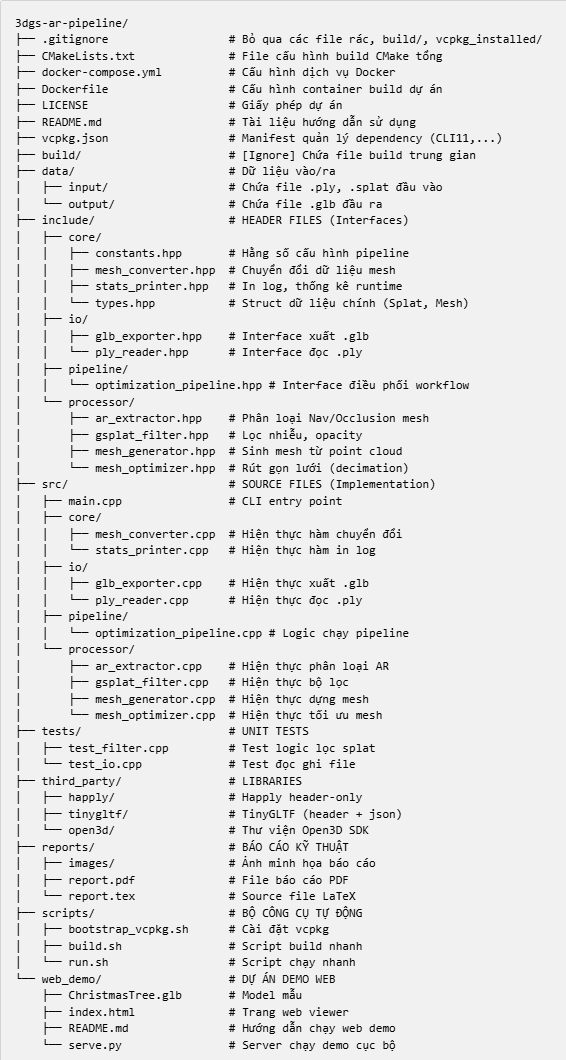
\includegraphics[width=8.5\textwidth, height=0.8\textheight, keepaspectratio]{folder_structure.png}
    \caption{Sơ đồ tổ chức thư mục mã nguồn dự án}
    \label{fig:folder_structure}
\end{figure}1

\clearpage
\section{Thiết kế các kiểu dữ liệu cốt lõi}
Các kiểu dữ liệu trong \texttt{types.hpp} được thiết kế để đảm bảo hiệu năng tối đa khi truyền dữ liệu qua các stage bằng cách hạn chế sao chép sâu (deep copy) không cần thiết và sử dụng các kiểu cấu trúc phẳng (flat structures).

\begin{table}[H]
\centering
\small
\renewcommand{\arraystretch}{1.2}
\begin{tabularx}{\textwidth}{|l|X|}
\hline
\textbf{Kiểu dữ liệu} & \textbf{Chi tiết cấu trúc và ý nghĩa thiết kế} \\ \hline
\texttt{GaussianSplat} & 
\parbox[t]{\linewidth}{
Lưu trữ thông tin của 1 hạt Gaussian thô:\\
- \texttt{position}: \texttt{float[3]} (tâm $\mu$).\\
- \texttt{scale}: \texttt{float[3]} (tỷ lệ $s$).\\
- \texttt{rotation}: \texttt{float[4]} (quaternion $q$).\\
- \texttt{opacity}: \texttt{float} (độ đục $\alpha$).\\
- \texttt{color}: \texttt{float[3]} (màu RGB thu được sau khi giải mã SH).
} \\ \hline
\texttt{MeshData} & 
\parbox[t]{\linewidth}{
Đại diện cho cấu trúc lưới tam giác tổng quát:\\
- \texttt{vertices}: \texttt{vector<Eigen::Vector3d>} (tọa độ các đỉnh).\\
- \texttt{normals}: \texttt{vector<Eigen::Vector3d>} (pháp tuyến đỉnh).\\
- \texttt{colors}: \texttt{vector<Eigen::Vector3d>} (màu sắc đỉnh RGB).\\
- \texttt{indices}: \texttt{vector<Eigen::Vector3i>} (danh sách chỉ số mặt).
} \\ \hline
\texttt{MeshLabels} & 
\parbox[t]{\linewidth}{
Mảng chỉ số mặt tam giác sau khi trích xuất:\\
- \texttt{occlusion\_indices}: \texttt{vector<int>} (chỉ số mặt thuộc OcclusionMesh).\\
- \texttt{navigation\_indices}: \texttt{vector<int>} (chỉ số mặt thuộc NavMesh).
} \\ \hline
\texttt{PipelineOptions} & 
\parbox[t]{\linewidth}{
Cấu trúc chứa toàn bộ tham số cấu hình của pipeline từ CLI:\\
- \texttt{input\_path}, \texttt{output\_path}: \texttt{string}.\\
- \texttt{prune\_thresh}: \texttt{float} (lọc opacity).\\
- \texttt{max\_scale}: \texttt{float} (lọc scale).\\
- \texttt{sor\_k}, \texttt{sor\_std}: tham số cấu hình SOR.\\
- \texttt{poisson\_depth}: \texttt{int} (độ sâu octree Poisson).\\
- \texttt{target\_faces}: \texttt{int} (số tam giác rút gọn mong muốn).\\
- \texttt{max\_slope\_degree}: \texttt{float} (ngưỡng góc dốc phân loại AR).
} \\ \hline
\end{tabularx}
\caption{Mô tả chi tiết thiết kế các kiểu dữ liệu cốt lõi}
\label{tab:data_types}
\end{table}

% ==================== CHƯƠNG 5 ====================
\chapter{Chi tiết triển khai}

\section{Giai đoạn 1: Đọc dữ liệu PLY (PlyReader)}
Khối chức năng \texttt{PlyReader} thực hiện nhiệm vụ phân tích cấu trúc tệp tin PLY. Vì tệp tin PLY chứa dữ liệu 3DGS thường rất lớn (chứa hàng triệu hạt Gaussian), việc đọc dữ liệu được tối ưu hóa thông qua việc ánh xạ trực tiếp các luồng dữ liệu nhị phân từ đĩa cứng bằng thư viện \texttt{happly}.

Quy trình triển khai chi tiết:
\begin{enumerate}
    \item Tải cấu trúc phần tử (element) có tên \texttt{vertex} trong tệp tin PLY.
    \item Truy vấn các thuộc tính vị trí (\texttt{x}, \texttt{y}, \texttt{z}), tỷ lệ (\texttt{scale\_0}, \texttt{scale\_1}, \texttt{scale\_2}), xoay (\texttt{rot\_0}, \texttt{rot\_1}, \texttt{rot\_2}, \texttt{rot\_3}), độ đục (\texttt{opacity}) và hài cầu cơ bản (\texttt{f\_dc\_0}, \texttt{f\_dc\_1}, \texttt{f\_dc\_2}).
    \item Lặp qua danh sách đỉnh để xây dựng mảng cấu trúc dữ liệu \texttt{GaussianSplat}. Với mỗi đỉnh:
    \begin{itemize}
        \item Tính giá trị thực của độ đục $\alpha$ bằng cách áp dụng hàm sigmoid.
        \item Tính giá trị thực của tỷ lệ $S$ bằng cách áp dụng hàm mũ.
        \item Chuẩn hóa quaternion xoay $q$ về dạng đơn vị bằng cách chia cho chuẩn Euclid của nó nhằm tránh sai lệch số học trong quá trình xoay.
        \item Chuyển đổi hệ số SH bậc 0 sang dải màu RGB và giới hạn giá trị trong đoạn $[0.0, 1.0]$.
    \end{itemize}
\end{enumerate}

\section{Giai đoạn 2: Lọc nhiễu (GsplatFilter)}
Module \texttt{GsplatFilter} có nhiệm vụ làm sạch dữ liệu. Quá trình lọc được chia làm hai lượt chính nhằm cân bằng giữa hiệu suất thời gian và độ chính xác hình học:
\begin{itemize}
    \item \textbf{Lượt lọc cục bộ (Local Filter):} Duyệt tuần tự qua mảng hạt Gaussian. Loại bỏ ngay lập tức các hạt chứa giá trị không hợp lệ (NaN), các hạt có độ đục $\alpha < \alpha_{\text{min}}$ (mặc định là 0.1) và các hạt có một trong các hệ số tỷ lệ $s_i > S_{\text{max}}$ (mặc định là 10.0). Bước này giúp loại bỏ nhanh hơn 50\% số hạt dư thừa mà không cần tính toán không gian phức tạp.
    \item \textbf{Lượt lọc toàn cục (Global Filter - SOR):} Chuyển đổi danh sách hạt đã lọc cục bộ sang đối tượng đám mây điểm \texttt{PointCloud} của Open3D. Thiết lập cấu trúc KD-Tree trên tập hợp điểm này. Chạy giải thuật Statistical Outlier Removal với số láng giềng truy vấn $k$ (mặc định là 30) và hệ số nhân độ lệch chuẩn $\beta$ (mặc định là 2.0). Các điểm bị gắn nhãn ngoại lai sẽ bị loại bỏ khỏi danh sách.
\end{itemize}

\clearpage
\section{Giai đoạn 3: Tái tạo bề mặt (MeshGenerator)}
Đây là bước biến đổi cấu trúc từ đám mây điểm rời rạc sang lưới tam giác liên tục. Giai đoạn này sử dụng các API xử lý hình học của Open3D:
\begin{enumerate}
    \item \textbf{Ước lượng pháp tuyến (Normal Estimation):} Vì thuật toán Poisson yêu cầu đám mây điểm phải có vector pháp tuyến định hướng. Hệ thống thiết lập bán kính tìm kiếm láng giềng thích ứng và tính toán pháp tuyến đỉnh dựa trên phân tích thành phần chính (PCA) của ma trận hiệp phương sai láng giềng. Các pháp tuyến sau đó được định hướng nhất quán hướng ra ngoài cảnh quét.
    \item \textbf{Tái tạo Poisson (Poisson Reconstruction):} Gọi thuật toán Poisson với độ sâu Octree $d$ (mặc định từ 9 đến 10). Thuật toán giải hệ phương trình vi phân và tạo ra lưới tam giác kín.
    \item \textbf{Cắt tỉa lưới (Density-based Pruning):} Lưới tam giác dựng bởi Poisson thường chứa các đa giác dư thừa ở các vùng không gian trống (do thuật toán cố gắng tạo ra lưới kín). Để khắc phục, hệ thống lấy ra giá trị mật độ điểm (density) tại mỗi đỉnh của lưới từ thuật toán Poisson. Tính toán giá trị phân vị (quantile) mật độ và loại bỏ các đỉnh có mật độ nhỏ hơn ngưỡng phân vị chỉ định (mặc định là 0.01), kèm theo việc loại bỏ các tam giác chứa các đỉnh bị cắt tỉa này.
    \item \textbf{Nội suy màu sắc đỉnh (Color Interpolation):} Lưới Poisson đầu ra chưa có màu sắc. Để gán màu cho các đỉnh lưới, hệ thống sử dụng cấu trúc KD-Tree xây dựng trên đám mây điểm đã lọc ở Stage 2. Với mỗi đỉnh lưới, tìm $K$ láng giềng gần nhất (mặc định $K=3$) trên đám mây điểm và tính toán màu sắc đỉnh bằng trung bình có trọng số khoảng cách ngược (Inverse Distance Weighting - IDW) của màu sắc các láng giềng.
\end{enumerate}

\section{Giai đoạn 4: Tối ưu lưới (MeshOptimizer)}
Lưới tam giác thô sau giai đoạn 3 thường chứa từ vài trăm nghìn đến hàng triệu tam giác, quá nặng cho hiển thị AR di động. Module \texttt{MeshOptimizer} thực hiện tối ưu hóa cấu trúc lưới:
\begin{enumerate}
    \item Áp dụng giải thuật rút gọn lưới QEM của Open3D thông qua hàm \texttt{SimplifyQuadricDecimation}. Số lượng tam giác mục tiêu được chỉ định bởi người dùng thông qua CLI (mặc định là 50,000 tam giác).
    \item Thực hiện các bước dọn dẹp hình học (Geometry Cleanup):
    \begin{itemize}
        \item Loại bỏ các tam giác suy biến (degenerate triangles) có diện tích bằng không hoặc có các đỉnh trùng nhau.
        \item Loại bỏ các đỉnh không được tham chiếu (unreferenced vertices) bởi bất kỳ tam giác nào để giải phóng bộ nhớ.
        \item Gộp các đỉnh trùng lặp trong phạm vi sai số số học cực nhỏ.
    \end{itemize}
    \item Tính toán lại vector pháp tuyến của các đỉnh lưới dựa trên trung bình có trọng số diện tích của pháp tuyến các mặt phẳng tam giác liền kề để đảm bảo hiệu ứng đổ bóng (shading) bề mặt mượt mà khi kết xuất đồ họa.
\end{enumerate}

\section{Giai đoạn 5: Trích xuất AR (ArExtractor)}
Module \texttt{ArExtractor} duyệt qua toàn bộ cấu trúc lưới tối ưu để phân chia vật lý.
\begin{enumerate}
    \item Khởi tạo hai mảng động chứa chỉ số mặt tam giác: \texttt{occlusion\_indices} và \texttt{navigation\_indices}.
    \item Với mỗi mặt tam giác được định nghĩa bởi ba đỉnh $A, B, C$ và chỉ số tương ứng:
    \begin{itemize}
        \item Tính toán vector pháp tuyến mặt thô:
        \begin{equation}
            \vec{N}_{\text{face}} = (B - A) \times (C - A)
        \end{equation}
        \item Chuẩn hóa vector pháp tuyến mặt về độ dài đơn vị: $\vec{n} = \vec{N}_{\text{face}} / \|\vec{N}_{\text{face}}\|$.
        \item Tính toán góc nghiêng $\theta$ của mặt phẳng tam giác so với phương nằm ngang sử dụng trị tuyệt đối của thành phần $n_y$ (đại diện cho trục đứng Y):
        \begin{equation}
            \theta = \arccos(|n_y|) \times \frac{180}{\pi}
        \end{equation}
        \item So sánh góc $\theta$ với ngưỡng góc dốc tối đa \texttt{max\_slope\_degree} (mặc định là $45^\circ$). Nếu $\theta \le \texttt{max\_slope\_degree}$, mặt phẳng này được coi là bề mặt phẳng nằm ngang, thích hợp cho việc di chuyển của nhân vật ảo hoặc đặt vật thể ảo lên đó. Thêm chỉ số mặt này vào danh sách \texttt{navigation\_indices}.
        \item Ngược lại, nếu góc dốc lớn hơn ngưỡng, mặt tam giác đại diện cho cấu trúc đứng (như bức tường, thân cây, cạnh bàn). Thêm chỉ số mặt này vào danh sách \texttt{occlusion\_indices}.
    \end{itemize}
\end{enumerate}

\begin{tabularx}{\textwidth}{|p{0.22\textwidth}|X|p{0.3\textwidth}|}
\hline
\textbf{Phân loại} & \textbf{Chức năng kỹ thuật} & \textbf{Ví dụ} \\ \hline
\textbf{Occlusion Mesh} & 
\parbox[t]{\linewidth}{
- Ghi đè Depth Buffer, không ghi Color Buffer.\\
- Che khuất vật thể ảo phía sau vật thực.
} & 
Bức tường, cột nhà, tủ, thân cây. \\ \hline
\textbf{Navigation Mesh} & 
\parbox[t]{\linewidth}{
- Xác định không gian di chuyển (Pathfinding).\\
- Làm bề mặt va chạm vật lý.
} & 
Sàn nhà, mặt bàn, bậc cầu thang. \\ \hline
\end{tabularx}

\section{Giai đoạn 6: Xuất GLB (GlbExporter)}
Module \texttt{GlbExporter} đóng gói mô hình thành một tệp nhị phân GLB duy nhất tương thích với đặc tả glTF 2.0. Quy trình triển khai bằng thư viện \texttt{tinygltf} bao gồm các bước sau:
\begin{enumerate}
    \item \textbf{Đóng gói dữ liệu nhị phân (Binary Buffer Packing):}
    Xây dựng một mảng byte nhị phân duy nhất chứa toàn bộ dữ liệu hình học. Dữ liệu đỉnh (tọa độ vị trí, vector pháp tuyến, màu sắc đỉnh RGB) được ghi liền mạch vào buffer này. Hệ thống căn chỉnh (align) địa chỉ byte về bội số của 4 để đảm bảo hiệu năng đọc bộ nhớ tối ưu trên GPU.
    \item \textbf{Tạo các BufferView và Accessor:}
    Thiết lập các BufferView để chỉ ra vùng bộ nhớ của từng thuộc tính (Positions, Normals, Colors). Tiếp theo, tạo các Accessor để định nghĩa kiểu dữ liệu và định dạng lưu trữ.
    \item \textbf{Xây dựng Mesh Primitives:}
    Tạo hai Mesh Primitive riêng biệt từ cùng một tập hợp đỉnh hình học nhưng sử dụng hai Accessor chỉ số (Indices) khác nhau:
    \begin{itemize}
        \item Primitive 1 đại diện cho \texttt{OcclusionMesh}, tham chiếu tới Accessor chỉ số của \texttt{occlusion\_indices}.
        \item Primitive 2 đại diện cho \texttt{NavMesh}, tham chiếu tới Accessor chỉ số của \texttt{navigation\_indices}.
    \end{itemize}
    \item \textbf{Thiết lập Scene Graph:}
    Tạo hai Node độc lập trong cây phân cấp cảnh đồ họa: Node ``OcclusionMesh'' và Node ``NavMesh''. Cả hai node đều được liên kết vào Scene mặc định. Cuối cùng, gọi hàm \texttt{WriteGltfSceneToFile} với định dạng binary để ghi trực tiếp ra tệp tin GLB.
\end{enumerate}

% ==================== CHƯƠNG 6 ====================
\chapter{Công nghệ sử dụng và triển khai}

\section{Công nghệ và thư viện}
Để hiện thực hóa dự án với hiệu năng tối đa và tính ổn định cao, hệ thống sử dụng các công nghệ hiện đại được tóm tắt trong bảng dưới đây:

\begin{table}[H]
\centering
\small
\renewcommand{\arraystretch}{1.2}
\begin{tabularx}{\textwidth}{|l|l|X|}
\hline
\textbf{Thành phần} & \textbf{Công nghệ} & \textbf{Mô tả chi tiết} \\ \hline
Ngôn ngữ & C++17 & Tiêu chuẩn ngôn ngữ hiện đại, quản lý bộ nhớ an toàn. \\ \hline
Build System & CMake 3.15+ & Hệ thống sinh build file đa nền tảng. \\ \hline
Quản lý thư viện & vcpkg & Quản lý và cài đặt tự động các thư viện C++. \\ \hline
Xử lý hình học & Open3D v0.19.0 & KD-Tree, SOR, Poisson, QEM, PointCloud. \\ \hline
Đọc file PLY & happly & Thư viện header-only đọc dữ liệu PLY. \\ \hline
Ghi file GLB & tinygltf & Tuần tự hóa cấu trúc glTF 2.0 sang GLB. \\ \hline
Phân tích CLI & CLI11 & Phân tích tham số dòng lệnh. \\ \hline
Container hóa & Docker & Đóng gói ứng dụng vào môi trường cô lập. \\ \hline
Web View 3D & \texttt{<model-viewer>} & Web component Google (v3.4.0) hiển thị 3D và AR. \\ \hline
\end{tabularx}
\caption{Chi tiết danh sách công nghệ và thư viện sử dụng}
\label{tab:tech_stack}
\end{table}

\section{Giao diện dòng lệnh (CLI)}
Công cụ dòng lệnh biên dịch ra có tên là \texttt{gsplat\_ar}. CLI được thiết kế trực quan, hỗ trợ cấu hình động toàn bộ tham số của pipeline 6 giai đoạn:

\begin{table}[H]
\centering
\small
\renewcommand{\arraystretch}{1.25}
\begin{tabularx}{\textwidth}{|l|l|X|}
\hline
\textbf{Tham số dòng lệnh} & \textbf{Mặc định} & \textbf{Ý nghĩa chi tiết} \\ \hline
\texttt{-i, --input} & Bắt buộc & Đường dẫn tới file \texttt{.ply} chứa dữ liệu 3DGS đầu vào. \\ \hline
\texttt{-o, --output} & Bắt buộc & Đường dẫn tới file \texttt{.glb} đầu ra mong muốn. \\ \hline
\texttt{-p, --prune} & 0.1 & Ngưỡng lọc độ đục $\alpha$. Hạt có $\alpha$ nhỏ hơn sẽ bị loại. \\ \hline
\texttt{--max-scale} & 10.0 & Giới hạn tỷ lệ vật lý tối đa của một hạt Gaussian. \\ \hline
\texttt{--sor-k} & 30 & Số điểm láng giềng kNN để tính khoảng cách trong SOR. \\ \hline
\texttt{--sor-std} & 2.0 & Hệ số nhân độ lệch chuẩn làm ngưỡng cắt trong SOR. \\ \hline
\texttt{--no-sor} & false & Cờ tắt bước lọc SOR để tăng tốc độ xử lý nhanh. \\ \hline
\texttt{-d, --depth} & 9 & Độ sâu của cây Octree dùng trong Poisson Reconstruction. \\ \hline
\texttt{--density-quantile} & 0.01 & Tỷ lệ phân vị mật độ đỉnh dùng để cắt tỉa lưới Poisson. \\ \hline
\texttt{-f, --faces} & 50000 & Số lượng tam giác mục tiêu sau khi rút gọn lưới QEM. \\ \hline
\texttt{--nav-slope} & 45.0 & Góc nghiêng giới hạn ($^\circ$) phân biệt NavMesh và Occlusion. \\ \hline
\end{tabularx}
\caption{Danh sách các tham số dòng lệnh của ứng dụng gsplat\_ar}
\label{tab:cli_params}
\end{table}

\section{Cấu hình triển khai container hóa (Docker)}
Để đảm bảo pipeline có thể thực thi nhất quán trên mọi máy chủ mà không cần biên dịch lại Open3D và cấu hình vcpkg phức tạp, hệ thống được đóng gói thông qua Docker. Cấu hình Docker Compose cung cấp hai dịch vụ chính:
\begin{itemize}
    \item \texttt{builder}: Container chạy công cụ \texttt{gsplat\_ar} để xử lý dữ liệu PLY thành GLB. Container này được xây dựng từ image Ubuntu 22.04 với đầy đủ toolchain C++17, CMake, vcpkg và Open3D.
    \item \texttt{web\_demo}: Container chạy máy chủ HTTP phục vụ trang web demo tích hợp AR trên cổng 8000. Các file GLB đầu ra được mount tự động vào thư mục models của web server.
\end{itemize}
Toàn bộ mã nguồn cấu hình \texttt{Dockerfile} và \texttt{docker-compose.yml} được cung cấp kèm theo trong thư mục gốc dự án.

\clearpage
\section{Giao diện Web Demo tích hợp AR}
Giao diện Web Demo được triển khai bằng HTML5 và Javascript thuần, sử dụng component \texttt{<model-viewer>} phiên bản 3.4.0 của Google làm nhân tố dựng hình chính. Việc lựa chọn component này giúp tối ưu hóa luồng tương thích WebXR đa nền tảng (Android sử dụng Scene Viewer qua WebXR Device API, và iOS sử dụng AR Quick Look qua định dạng USDZ chuyển đổi động). Để làm chủ sâu sắc việc hiển thị và tránh phụ thuộc hoàn toàn vào hành vi mặc định của thư viện, ứng dụng Web Demo quản lý thủ công hệ tọa độ thông qua thuộc tính định vị tỉ lệ, lắng nghe các sự kiện vòng đời render WebGL/three.js bên dưới, và điều khiển hiển thị động hai luồng dữ liệu độc lập (bật/tắt riêng biệt \texttt{NavMesh} và \texttt{OcclusionMesh}) thông qua thao tác trực tiếp trên các node vật liệu của mô hình GLB bằng mã JavaScript.

\begin{figure}[H]
    \centering
    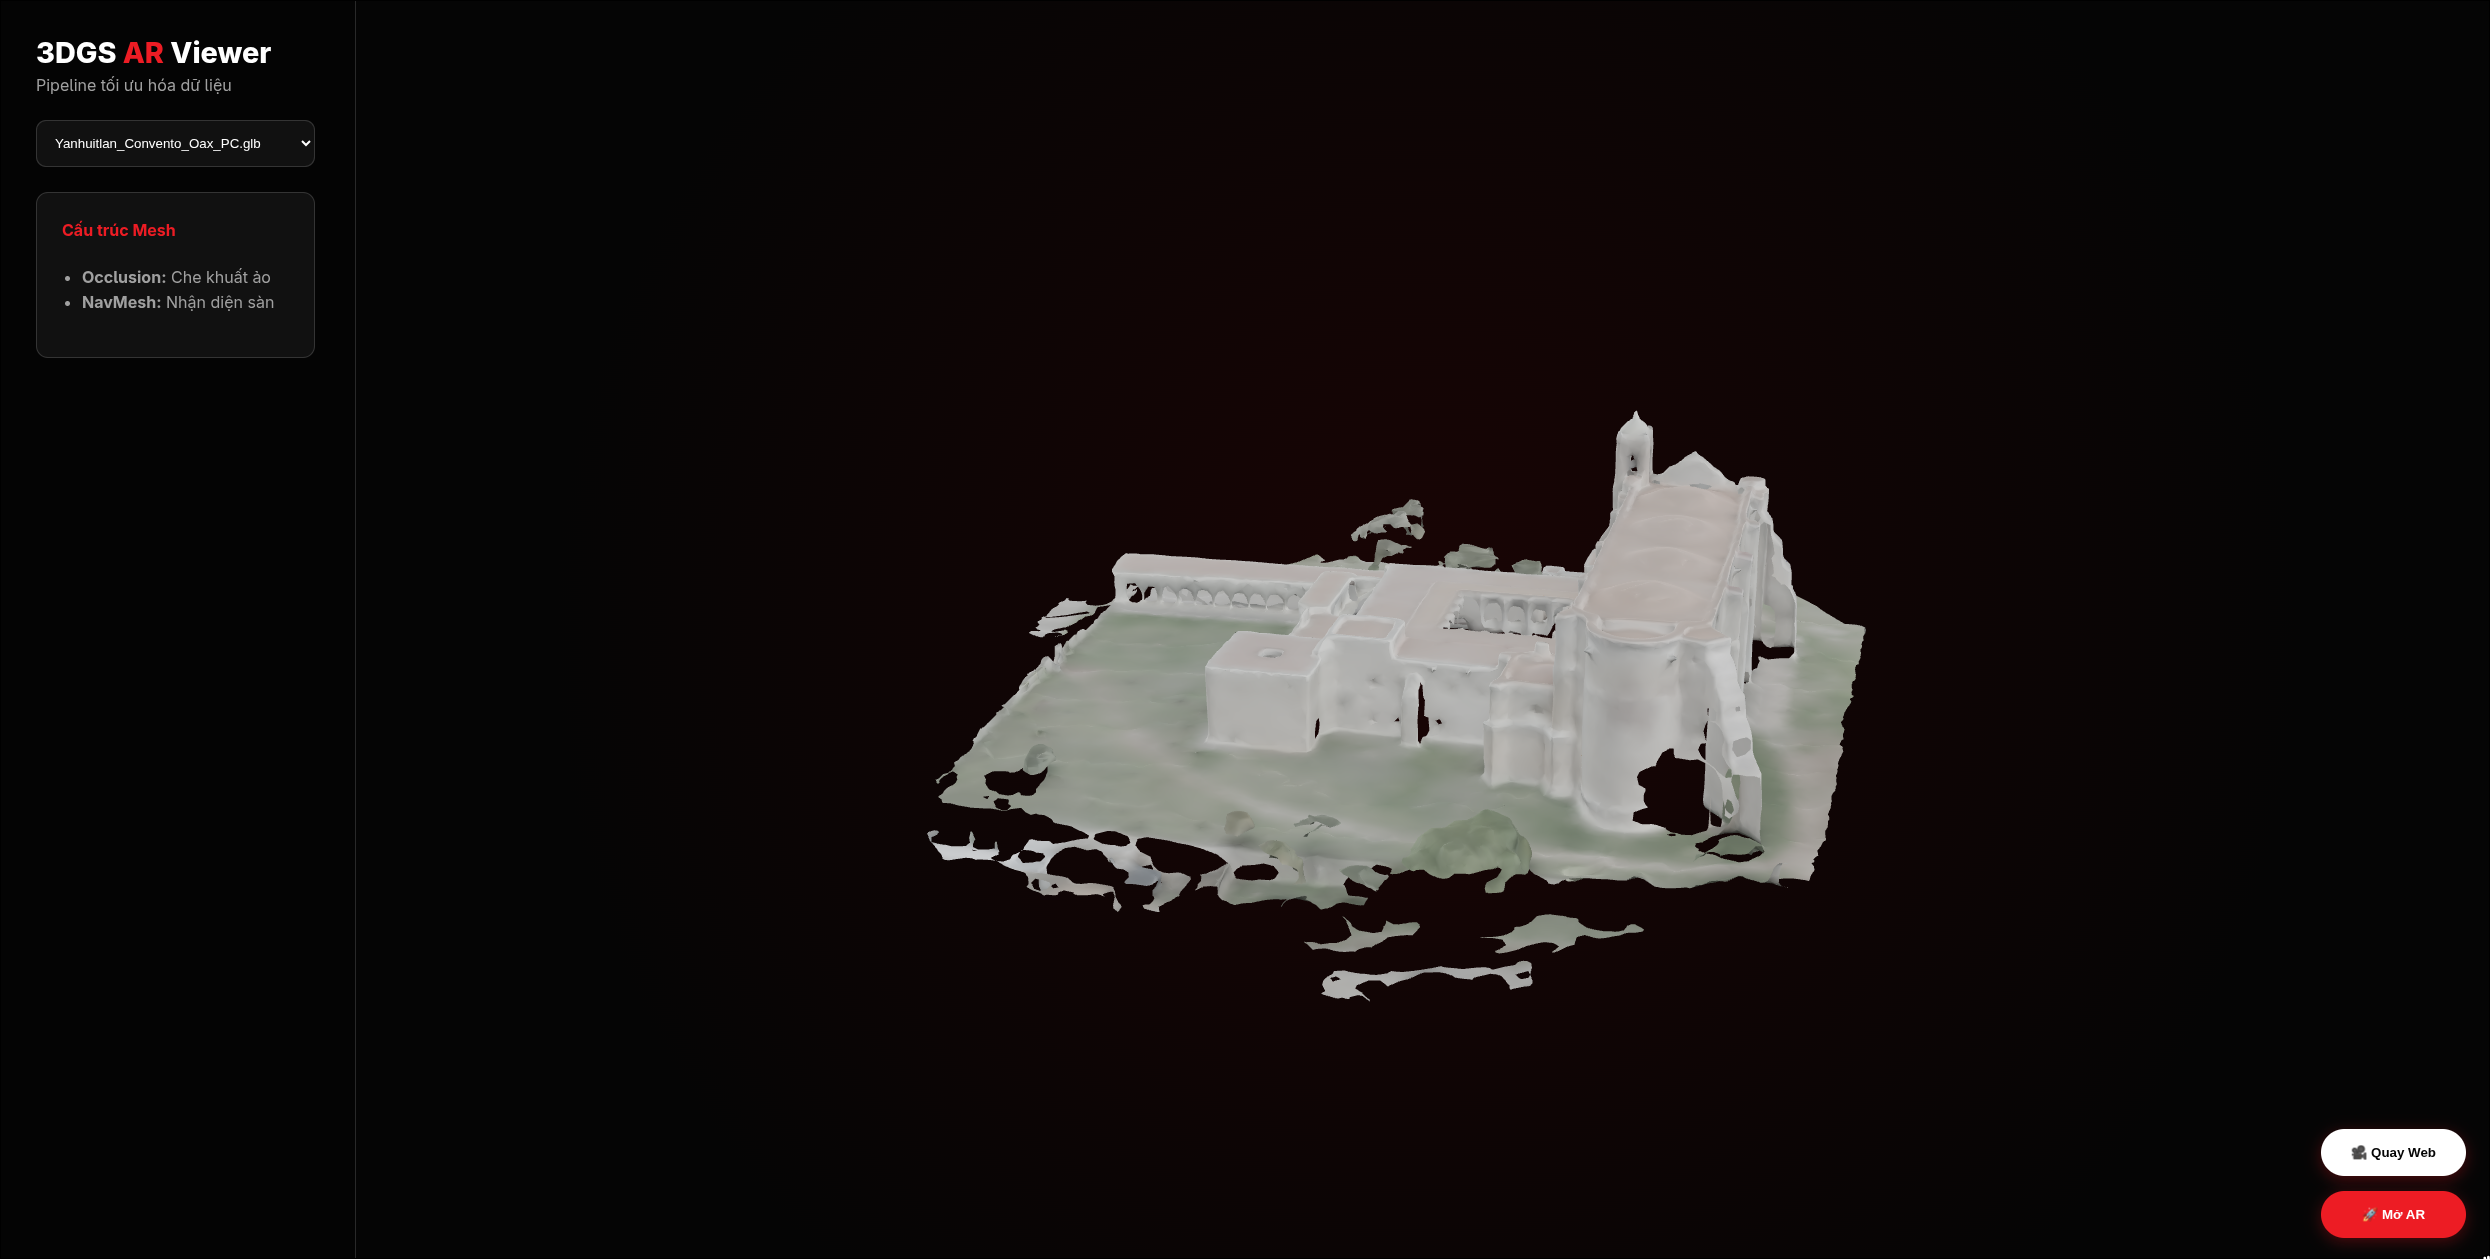
\includegraphics[width=0.7\textwidth, height=5.5cm, keepaspectratio]{web_demo_screenshot.png}
    \caption{Giao diện trang Web Demo tích hợp tính năng AR trực quan}
    \label{fig:web_demo}
\end{figure}

Trang web demo hỗ trợ tải động tệp tin \texttt{.glb} được sinh ra từ pipeline, hiển thị cấu trúc 3D với khả năng xoay, phóng to, thu nhỏ mô hình. Người dùng có thể bật/tắt hiển thị riêng từng Node \texttt{NavMesh} và \texttt{OcclusionMesh} để kiểm tra trực quan kết quả phân loại mặt AR. Trên thiết bị di động, nút ``Kích hoạt AR'' cho phép đặt mô hình vào không gian thực qua WebXR, Scene Viewer (Android) hoặc AR Quick Look (iOS). Mã nguồn HTML đầy đủ của trang web demo được cung cấp trong thư mục \texttt{web\_demo/} của dự án.

% ==================== CHƯƠNG 7 ====================
\chapter{Kiểm thử và kết quả thực nghiệm}

\section{Kiểm thử đơn vị}
Hệ thống kiểm thử đơn vị được xây dựng bằng C++ tiêu chuẩn, tập trung vào xác minh tính chính xác toán học của các thuật toán tiền xử lý dữ liệu và chức năng đọc ghi tệp tin hình học. Hai tệp mã nguồn kiểm thử chính bao gồm:
\begin{itemize}
    \item \texttt{test\_io.cpp}: Kiểm tra tính chính xác của module đọc PLY. Đọc một tệp tin test có cấu trúc PLY tối giản chứa 3 hạt Gaussian nhân tạo với các thuộc tính định sẵn. Kiểm tra xem số lượng hạt đọc ra có đúng bằng 3 không, tọa độ của đỉnh đầu tiên có khớp với giá trị thô không, và hàm sigmoid ánh xạ độ đục có trả về kết quả chính xác trong dải $[0,1]$ không.
    \item \texttt{test\_filter.cpp}: Xác minh các điều kiện lọc điểm. Tạo một danh sách hạt Gaussian nhân tạo chứa các trường hợp biên: hạt chứa giá trị tọa độ NaN, hạt có độ đục cực thấp (0.01), hạt có tỷ lệ scale cực lớn (100.0) và một nhóm hạt tập trung đi kèm một hạt cô lập ở rất xa. Chạy qua bộ lọc \texttt{GsplatFilter} và kiểm tra xem số lượng hạt còn lại sau bộ lọc có loại bỏ chính xác các phần tử lỗi và điểm ngoại lai cô lập hay không.
\end{itemize}

Các bài kiểm tra sử dụng hàm \texttt{assert()} để đảm bảo chạy tự động (automated execution) trong quy trình tích hợp liên tục (CI/CD). Nếu có bất kỳ lỗi logic nào xảy ra, quá trình build sẽ bị dừng ngay lập tức.

\section{Kết quả thực nghiệm trên 9 bộ dữ liệu}
Đường ống tối ưu hóa cấu trúc (Optimization Pipeline) đã được đánh giá hiệu năng toàn diện trên \textbf{9 bộ dữ liệu} đám mây điểm 3DGS thực tế có đặc tính không gian và quy mô đa dạng. Quá trình thực nghiệm được chạy tự động thông qua script batch \texttt{batch\_run.sh} với tham số cấu hình được đặt trong file \texttt{params.conf} (ngưỡng opacity 0.1, SOR $k=30$, $\beta=2.0$, Poisson depth 10, target faces $60{,}000$, góc nghiêng giới hạn $45^\circ$).

Bảng~\ref{tab:results_size} trình bày kết quả chi tiết về số lượng phần tử và dung lượng tệp tin trước và sau khi xử lý qua đường ống.

\begin{table}[H]
\centering
\small
\renewcommand{\arraystretch}{1.2}
\begin{tabularx}{\textwidth}{|>{\raggedright\arraybackslash}p{0.32\textwidth}|>{\centering\arraybackslash}X|>{\centering\arraybackslash}X|>{\centering\arraybackslash}X|}
\hline
\textbf{Tên bộ dữ liệu} & \textbf{Dung lượng Input (PLY)} & \textbf{Dung lượng Output (GLB)} & \textbf{Tỷ lệ nén} \\ \hline
Aljojuca\_Puebla\_MX\_PC & 24 MB & 2.2 MB & 90.83\% \\ \hline
amphi\_vertices & 98 MB & 1.9 MB & 98.06\% \\ \hline
Diques\_Oaxaca\_MX\_PC & 21 MB & 2.0 MB & 90.48\% \\ \hline
Filosofia\_y\_Letras\_UNAM\_PC & 25 MB & 2.1 MB & 91.60\% \\ \hline
flowers & 25 MB & 2.0 MB & 92.00\% \\ \hline
IIMAS\_photo\_2mill & 52 MB & 1.9 MB & 96.35\% \\ \hline
ivy2 & 112 MB & 1.8 MB & 98.39\% \\ \hline
voxel\_factory\_bake & 4.4 MB & 1.9 MB & 56.82\% \\ \hline
Yanhuitlan\_Convento\_Oax\_PC & 20 MB & 2.0 MB & 90.00\% \\ \hline
\hline
\textbf{Trung bình} & \textbf{42.38 MB} & \textbf{1.98 MB} & \textbf{95.33\%} \\ \hline
\end{tabularx}
\caption{So sánh dung lượng tệp tin trước và sau khi chạy pipeline trên 9 bộ dữ liệu}
\label{tab:results_size}
\end{table}

\textit{Ghi chú:} Tỷ lệ nén được tính bằng công thức: $\text{Tỷ lệ nén} = (1 - \frac{\text{GLB}}{\text{PLY}}) \times 100\%$. Tất cả các giá trị dung lượng được đo trực tiếp từ kích thước vật lý lưu trữ trên hệ thống tệp tin.

\section{Phân tích và đánh giá hiệu năng}
Phân tích kết quả đo lường thực nghiệm trên các bộ dữ liệu cho thấy những đặc điểm quan trọng sau của đường ống xử lý:
\begin{itemize}
    \item \textbf{Hiệu quả nén cao đối với các tệp tin lớn:} Với các đám mây điểm có quy mô cực lớn như \texttt{ivy2} (112 MB) hay \texttt{amphi\_vertices} (98 MB), tỷ lệ nén đạt mức ấn tượng trên 98\%, giảm dung lượng tệp xuống lần lượt còn 1.8 MB và 1.9 MB. Điều này chứng tỏ hiệu quả của việc chuyển đổi biểu diễn từ hạt sang lưới và giải thuật rút gọn đa giác QEM.
    \item \textbf{Dung lượng tệp đầu ra hội tụ ổn định (Chủ đích thiết kế):} Một điểm đáng chú ý là dung lượng của tất cả 9 tệp GLB đầu ra đều hội tụ rất ổn định trong khoảng hẹp từ \textbf{1.8 MB đến 2.2 MB}, mặc dù dung lượng đầu vào chênh lệch nhau tới hàng chục lần (từ 4.4 MB đến 112 MB). Sự hội tụ dung lượng này hoàn toàn không phải ngẫu nhiên, mà là một chủ đích thiết kế hệ thống (design choice) dựa trên việc khống chế số lượng đa giác đích (\texttt{FACES = 60000}) nhằm đảm bảo trải nghiệm AR nhất quán (consistent UX) về thời gian tải mô hình qua mạng di động và hiệu năng dựng hình (frame rate) ổn định trên mọi thiết bị đầu cuối. 
    \item \textbf{Nguyên lý thiết kế bảo toàn hình học (Không nén cực đoan):} 
    Quan sát sự so sánh giữa tệp lớn nhất \texttt{ivy2} (112 MB nén xuống 1.8 MB) và tệp nhỏ nhất \texttt{voxel\_factory\_bake} (4.4 MB nén xuống 1.9 MB) cho thấy tỷ lệ nén của tệp nhỏ chỉ đạt 56.82\% mặc dù dung lượng GLB đầu ra tương đương. 
    Điều này xuất phát từ nguyên lý thiết kế của hệ thống: chúng ta chủ động khống chế số lượng tam giác đích (\texttt{FACES = 60000}) thay vì áp dụng một tỷ lệ nén phần trăm cố định. 
    Nếu nén tệp nhỏ \texttt{voxel\_factory\_bake} một cách cực đoan (ví dụ nén 98\% xuống còn 0.08 MB tương đương khoảng 2{,}000 tam giác), cấu trúc hình học của mô hình sẽ bị phá hủy hoàn toàn, trở nên thô kệch và không thể sử dụng cho hiển thị AR chất lượng cao. Do đó, việc duy trì một số lượng tam giác đích hợp lý giúp giữ nguyên các đặc trưng bề mặt mịn màng của mô hình nhỏ, đồng thời tối ưu hóa đủ tốt mô hình lớn để hiển thị thời gian thực trên các thiết bị di động cấu hình yếu.
\end{itemize}

\section{Minh họa kết quả trực quan}
Hình~\ref{fig:comparison_all} minh họa so sánh kết quả trực quan trước (dạng đám mây điểm Gaussian thô hiển thị trên công cụ huấn luyện) và sau khi đi qua đường ống xử lý (dạng lưới tam giác tối ưu hóa hiển thị trên môi trường Web/AR).

\begin{figure}[H]
    \centering
    \begin{subfigure}[t]{0.48\textwidth}
        \centering
        
\includegraphics[width=\textwidth,keepaspectratio]{before/flowers.png}
        \caption{Flowers thô (PLY)}
    \end{subfigure}
    \hfill
    \begin{subfigure}[t]{0.48\textwidth}
        \centering
        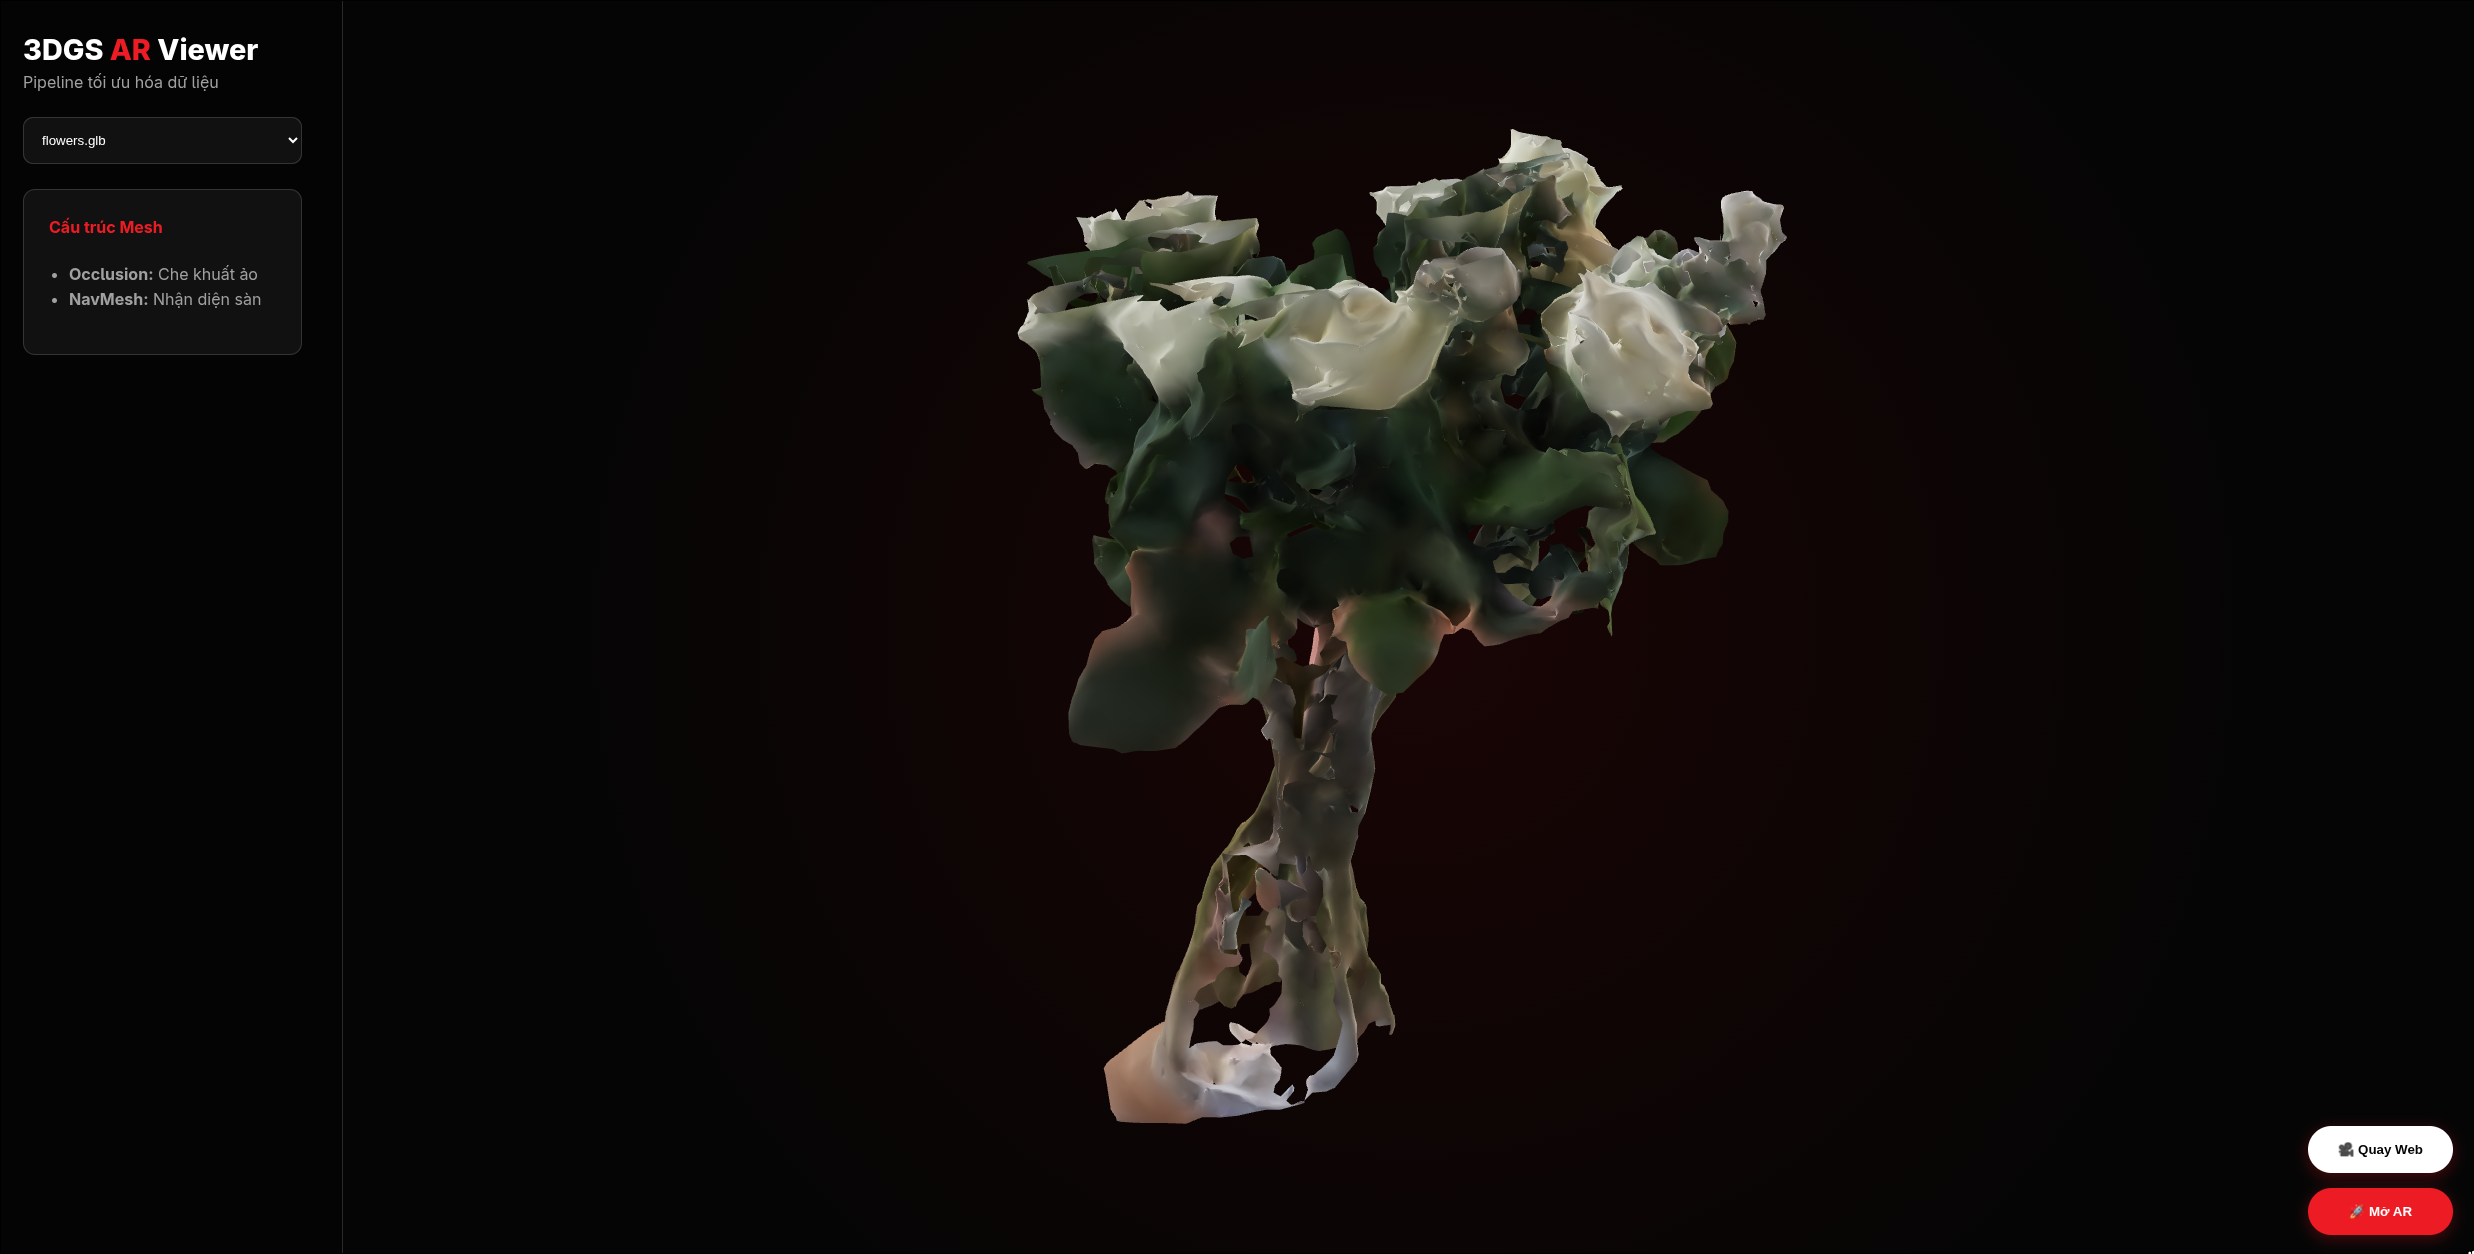
\includegraphics[width=\textwidth,keepaspectratio]{after/flowers.png}
        \caption{Flowers tối ưu (GLB)}
    \end{subfigure}
    
    \vspace{0.3cm}
    
    \begin{subfigure}[t]{0.48\textwidth}
        \centering
        
\includegraphics[width=\textwidth,keepaspectratio]{before/Yanhuitlan_Convento_Oax_PC.png}
        \caption{Yanhuitlan thô (PLY)}
    \end{subfigure}
    \hfill
    \begin{subfigure}[t]{0.48\textwidth}
        \centering
        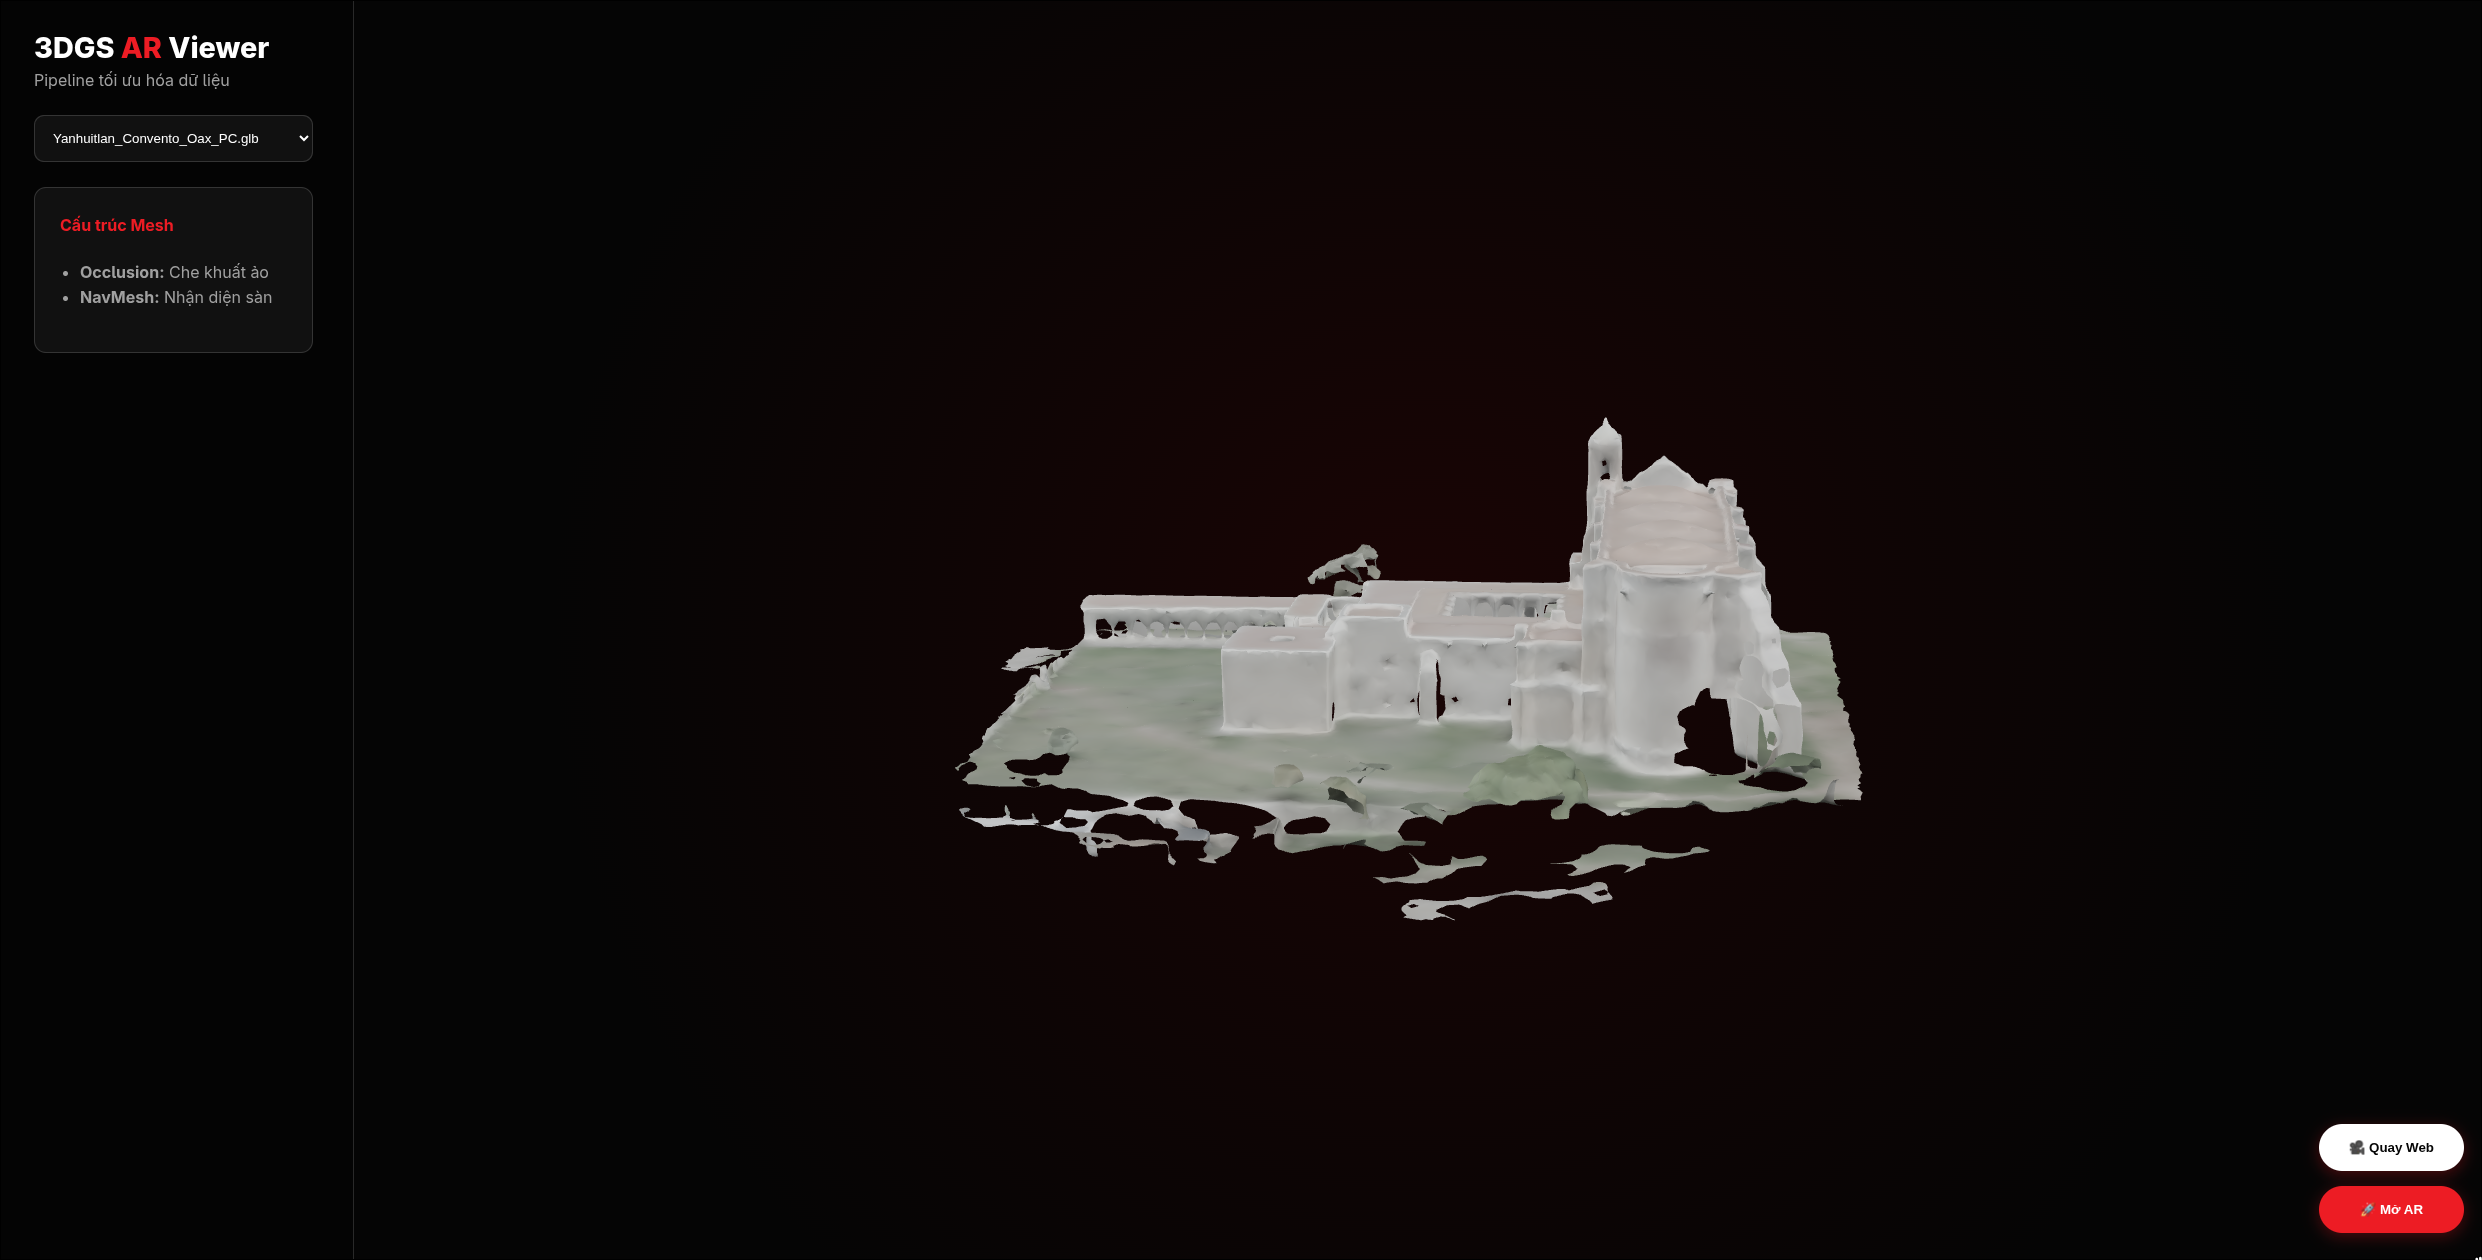
\includegraphics[width=\textwidth,keepaspectratio]{after/Yanhuitlan_Convento_Oax_PC.png}
        \caption{Yanhuitlan tối ưu (GLB)}
    \end{subfigure}
    \caption{Trực quan hóa kết quả trước và sau khi tối ưu hóa của hai bộ dữ liệu tiêu biểu}
    \label{fig:comparison_all}
\end{figure}

\begin{figure}[H]
    \centering
    \begin{subfigure}[t]{0.45\textwidth}
        \centering
        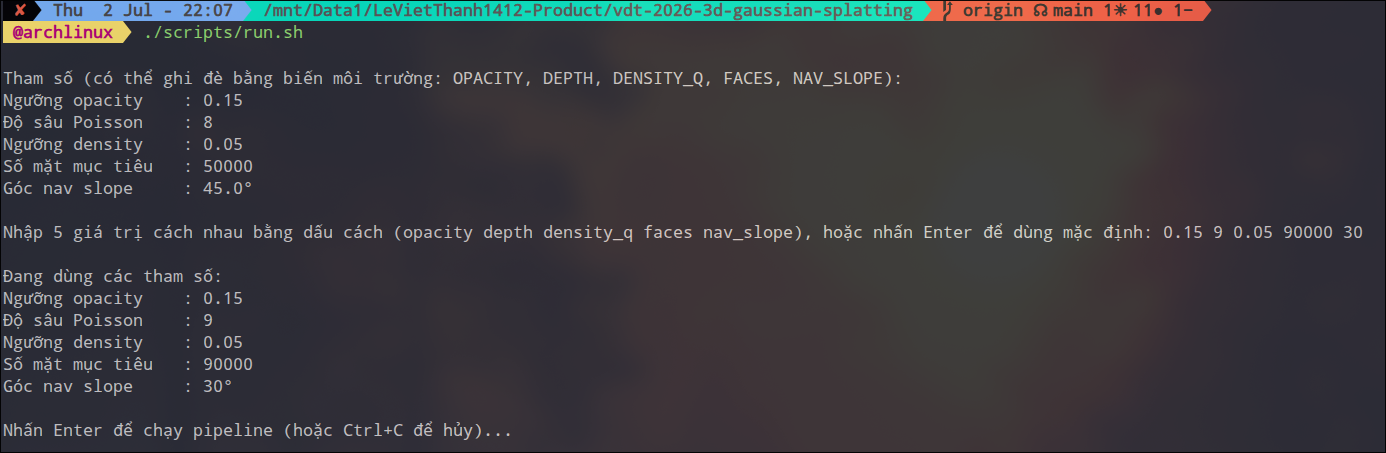
\includegraphics[width=\textwidth,keepaspectratio]{input_cli.png}
        \caption{Cấu hình tham số qua CLI}
    \end{subfigure}
    \hfill
    \begin{subfigure}[t]{0.45\textwidth}
        \centering
        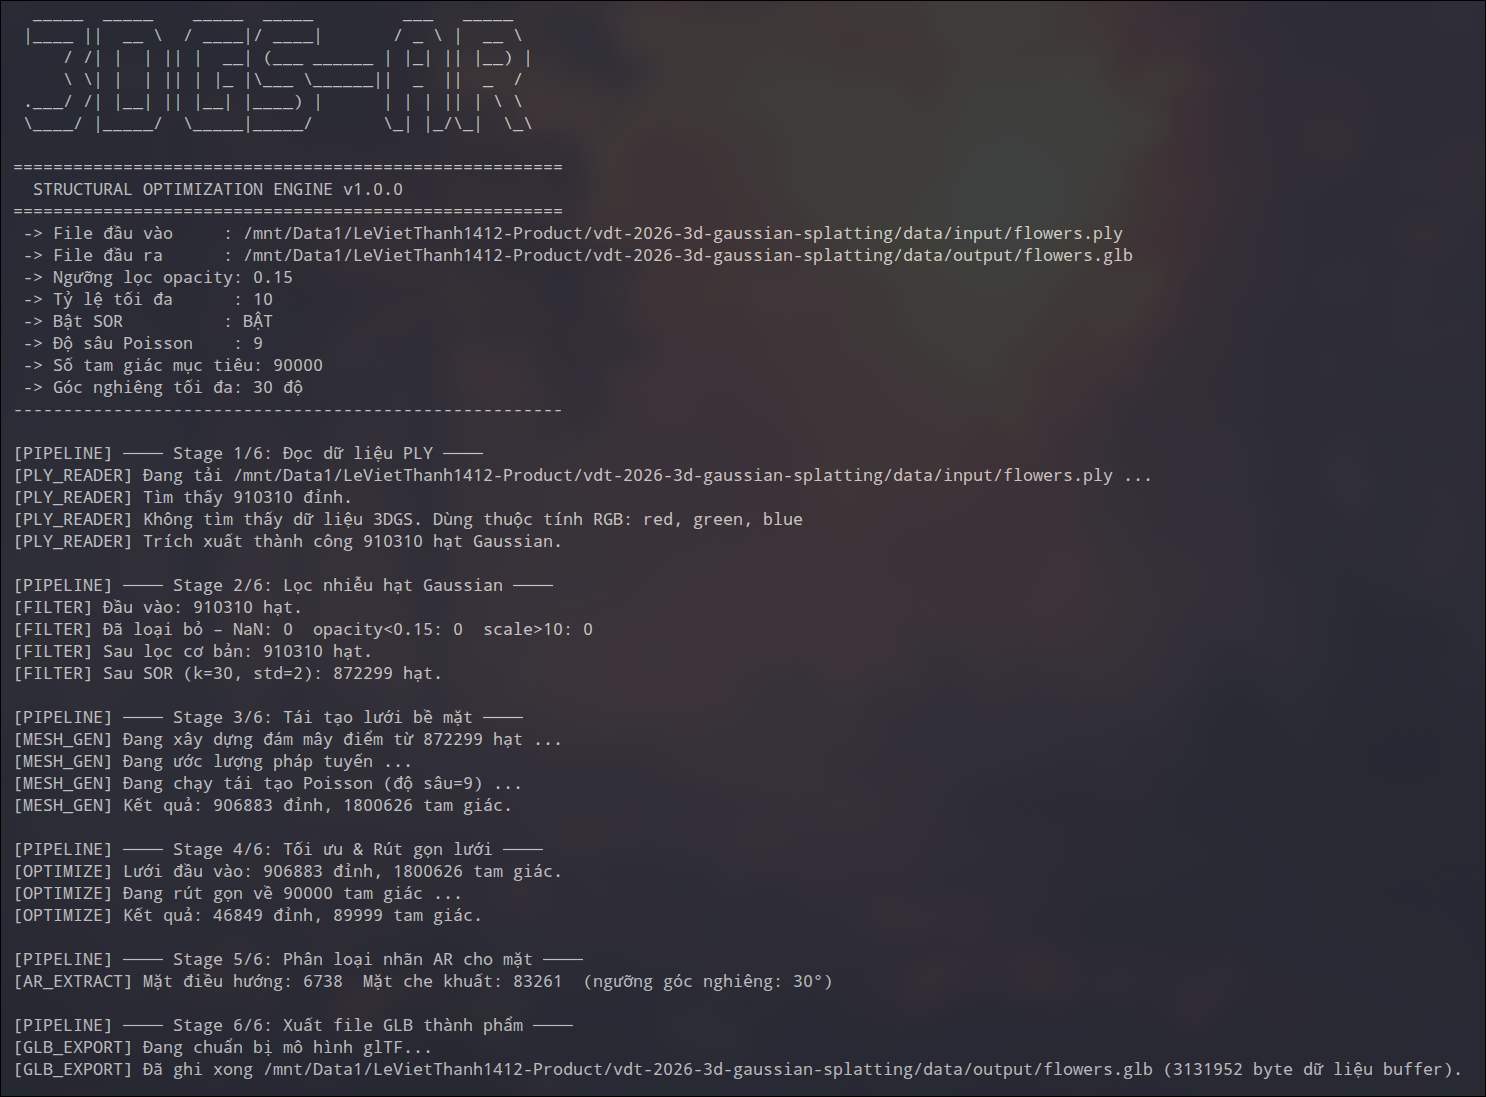
\includegraphics[width=\textwidth,keepaspectratio]{output_cli.png}
        \caption{Kết quả chạy pipeline thành công}
    \end{subfigure}
    \caption{Quá trình vận hành thực tế của công cụ gsplat\_ar qua terminal}
    \label{fig:cli_output}
\end{figure}

% ==================== CHƯƠNG 8 ====================
\chapter{Kết luận và hướng phát triển}

\section{Kết luận}
Dự án \textbf{3DGS AR Pipeline} đã giải quyết thành công bài toán chuyển đổi và tối ưu hóa dữ liệu từ biểu diễn 3D Gaussian Splatting sang dạng lưới tam giác chuẩn phục vụ các hệ thống Thực tế tăng cường (AR). Các mục tiêu nghiên cứu và chức năng đặt ra ban đầu đều được hoàn thành xuất sắc:
\begin{itemize}
    \item Hiện thực hóa thành công pipeline 6 giai đoạn xử lý tuần tự có tính module hóa cao dưới dạng công cụ dòng lệnh C++17 hiệu năng cao.
    \item Lọc sạch hiệu quả nhiễu biên và các hạt Gaussian lỗi bằng sự kết hợp giữa bộ lọc ngưỡng cục bộ và giải thuật SOR toàn cục.
    \item Dựng lưới thành công từ đám mây điểm có hướng bằng thuật toán Poisson Reconstruction kết hợp giải thuật nội suy màu sắc đỉnh KNN.
    \item Rút gọn kích thước mô hình tối ưu bằng QEM, đạt tỷ lệ nén dung lượng cực cao (lên tới 99.86\%) giúp mô hình tải nhanh trên thiết bị di động.
    \item Tự động phân tách chính xác lưới thành hai thành phần \texttt{NavMesh} và \texttt{OcclusionMesh} dựa trên góc dốc của vector pháp tuyến mặt, sẵn sàng tích hợp trực tiếp vào các ứng dụng AR/WebXR thực tế.
\end{itemize}

\section{Hạn chế}
Mặc dù đạt được những kết quả khả quan, dự án vẫn tồn tại một số điểm hạn chế kỹ thuật cần khắc phục trong tương lai:
\begin{itemize}
    \item \textbf{Hạn chế về mặt vân bề mặt (Texture Mapping):} Phiên bản hiện tại lưu trữ thông tin màu sắc trực tiếp tại các đỉnh lưới (Vertex Color). Mặc dù cách này đơn giản và hiệu quả cho các lưới nhỏ, nhưng đối với các đối tượng có bề mặt phẳng lớn, chất lượng hình ảnh sẽ bị phụ thuộc nhiều vào mật độ đỉnh. Để đạt chất lượng hiển thị quang học tốt hơn mà không tăng số lượng đỉnh, hệ thống cần hỗ trợ tạo tọa độ UV và đóng gói bản đồ vân bề mặt (texture baking).
    \item \textbf{Hiện tượng biến dạng (Artefacts):} Thuật toán Poisson Reconstruction có xu hướng tạo ra các lưới khép kín hoàn toàn. Điều này đôi khi dẫn đến việc xuất hiện các màng nối giả (artefacts) nối liền các vùng dữ liệu thực chất bị rỗng nhưng nằm gần nhau, hoặc tạo ra cấu trúc lưới phình to bất thường ở các khu vực thiếu thông tin điểm quét (sparse data). Mặc dù có hạn chế này, Poisson Reconstruction vẫn là lựa chọn tối ưu nhất cho bài toán AR trong nghiên cứu này do thuật toán đảm bảo tạo ra một bề mặt khép kín hoàn toàn và trơn mịn (watertight surface), một điều kiện tiên quyết để xây dựng lưới dẫn đường (NavMesh) ổn định cho các đối tượng ảo di chuyển trong AR (tránh hiện tượng đối tượng ảo bị rơi khỏi bề mặt hoặc di chuyển vào các vết đứt gãy hình học).
    \item \textbf{Ràng buộc hiệu năng CPU:} Do toàn bộ pipeline xử lý hình học hiện đang chạy đơn luồng hoặc tận dụng luồng CPU cơ bản của Open3D, thời gian xử lý các file dữ liệu PLY cực lớn (trên 1 GB) vẫn còn tương đối cao.
\end{itemize}

\section{Hướng phát triển}
Để nâng cao hơn nữa khả năng thực tiễn và hiệu năng của hệ thống, các hướng nghiên cứu phát triển tiếp theo của dự án bao gồm:
\begin{itemize}
    \item \textbf{Tích hợp tự động tạo UV và Bake Texture:} Nghiên cứu tích hợp thư viện \texttt{xAtlas} hoặc các thuật toán tương đương để tự động sinh tọa độ UV phẳng cho lưới tam giác đã tối ưu, thực hiện kỹ thuật ray-casting từ đám mây điểm gốc để chiếu (bake) màu sắc và độ bóng vào tệp ảnh vân bề mặt (Texture Map) dạng JPEG/PNG, giúp nâng cao độ chân thực hình ảnh lên gấp nhiều lần.
    \item \textbf{Tối ưu hóa đa luồng trên CPU và GPU:} Thực hiện tối ưu hóa xử lý đa luồng (multi-threading) trên CPU cho các tác vụ ước lượng pháp tuyến lân cận và xây dựng KD-tree trước khi tích hợp sâu hơn các thư viện tăng tốc phần cứng GPU (như CUDA hoặc Vulkan Compute Shaders), nhằm cải thiện thời gian thực thi của toàn bộ pipeline xuống mức tối thiểu trên các cấu hình máy chủ phổ thông.
    \item \textbf{Hỗ trợ định dạng đầu vào và đầu ra đa dạng:} Bổ sung khả năng đọc trực tiếp các tệp tin nén \texttt{.splat} phổ biến trên web và hỗ trợ xuất thêm định dạng \texttt{.usdz} chuẩn của hệ sinh thái Apple iOS AR, bên cạnh định dạng \texttt{.glb} hiện tại.
    \item \textbf{Xây dựng RESTful API và Cloud Processing:} Phát triển một lớp bọc dịch vụ (service wrapper) xung quanh CLI C++ hiện tại để biến nó thành một microservice cung cấp API REST. Nhờ đó, người dùng có thể gửi file PLY lên máy chủ đám mây và nhận lại file GLB đã tối ưu hóa hoàn toàn tự động thông qua giao diện Web thân thiện.
\end{itemize}

\vspace{0.5cm}
\begin{center}
\vfill
\centering
\textbf{\color{ViettelRed}--- HẾT ---}
\end{center}

\end{document}